\chapter{Architecture as Interface - A Review of Spatial Interactions in Mediated Public Spaces}
\label{chapterlabel3}

%%%%%%%%%%%%%%%%%%%%%%%%%%%%%

\section*{Chapter summary}

In this chapter, I review the background of my research while referring to sources from architectural theory and research into interactive systems specifically into Interaction Design. I will illustrated this background with relevant applied projects. My particular focus will be on the relationship between the physical components that constitute interactive and large electronic surfaces, the spatial setting they are situated in and the interactions released. I will provide insights into the notion of public space, particularly looking at what constitutes a shared encounter and its spatio-temporal process. From there I will consider technology mediated interactions and an investigation to clarify what I mean by an extended notion of interfaces, their dependency on surfaces and the relevance of the spatial context. I will look at existing socio-spatial interaction frameworks derived from HCI research in the domain of public displays. This will then be followed by an overview of research and practice of case studies ranging from building projections to media architecture. Finally I will introduce the neologism Sentiment Architectures in anticipation of the case study of this dissertation. In the discussion I will argue that designing for a lively built environment needs to start with an understanding of the types of interactions one aims to stimulate, which today also demands a clear positioning towards the role of digital media technologies.  

Keywords: interactions, interfaces, surfaces, space

\newpage


%%%%%%%%%%%%%%%%%%%%%%%%%%%%%


\section{The Notion of Public Space}

\textit{Designing for people} (Dreyfuss, 1955) in the 20th century was characterised by Cartesian methods to map the physical needs of humans. Architects and designers such as LeCorbusier (Le Modulor), or Neufert (2002) surveyed human ergonomics to suggest design principles for an anthropometric scale based on Vitruv's early considerations of the human body (reference). Despite the acknowledgement of the human anatomy in architecture, human behaviour has been widely ignored. Architectural visions exploded in scale (Fig.\ref{RadiantCity}) whilst the need for a carefully thought of public space was widely ignored.

%%%%%%%%%%%%%%%%%%%%%%%%%%%%%

\begin{figure}[h] 
\centering
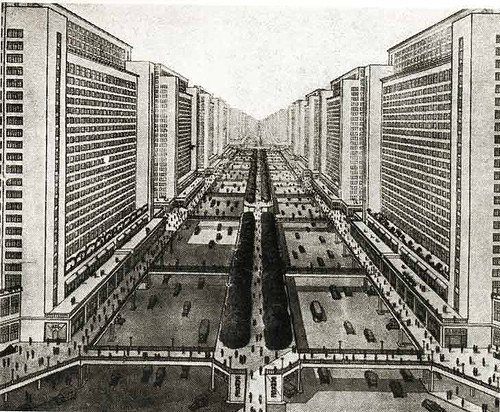
\includegraphics[width=10cm]{Illustrations/ville_radieuse.jpg}
\caption [The Radiant City, LeCorbusier (1924)] {LeCorbusier's large scale vision of a \textit{Radiant City} \index{Radiant City (1924)} introduced in 1924 suggested high density housing in form of monumental building blocks as a radical concept for a new quality of life. Large scale and repetitive architectural form refused to acknowledge the human scale and the characteristics of a vibrant public space.}
\label{RadiantCity}
\end{figure}

%%%%%%%%%%%%%%%%%%%%%%%%%%%%%

%\begin{singlespace}
%	\leftskip2.3em
%		\rightskip\leftskip
%			\textit{\small In her seminal book The Public Realm: Exploring the City’s Quintessential Social Territory, sociologist Lyn H. Lofland defines the public realm as that social entity within the physical settings of a city that is made up of interactions between  strangers—a successful public realm enables human interaction to take place. 
%} 	
%\end{singlespace}

%%%%%%%%%%%%%%%%%%%%%%%%%%%%%
 
Jane Jacobs \index{Jane Jacobs (1916-2006)} has been one of the early theorists who aimed to understand what constitutes public urban spaces.
Her book, \textit{The Death and Life of Great American Cities} (Jacobs 1961), is full of criticism on the then predominant post war urban planning, urban renewal and architecture. 
Rather than advocating for a particular architectural style Jacobs instead took a close look at the social behaviour of citizens in their local neighbourhoods. 
Jacobs' methodology was to conduct careful observations and conversations with residents in local neighbourhoods. 
She came to the conclusion that streets are the very essence of the city. 
Jacobs observed that the replacement of existing sound urban areas through up-scaling the built environment with residential super blocks, skyscrapers, shopping centres, monumental cultural centres and motorways, in other words the separation of function as proposed by Le Corbusier, led to the decline of former habitable areas, a lack of safety and the increase of poverty (Jacobs, 1961: 23-33).

Then in the 1970s \textit{The Street Life Project} \index{The Street Life Project (1980)} under the leadership of William H. Whyte \index{William H. Whyte (1917-1999)} systematically studied crowding on the streets of New York (Fig. \ref{fig:Whyte}). His research was driven by the question why some public spaces are more popular amongst dwellers than others. The observed imbalance of use in public space suggested practical implications \smalltodo[size=\footnotesize]{What are the practical implications? Could go in the appendix?.} towards a more liveable urban environment\cite{Whyte_1980} \footnote{In addition to the published book about the work conducted by \textit{The Street Live Project} a documentary has been released that clearly demonstrates the applied observations methods: \url{https://vimeo.com/111488563} [accessed 25.07.2016]}.


A comprehensive collection of attributes that describes what makes a great place originates from the non-profit-organisation \textit{Project for Public Spaces} \footnote{\url{http://www.pps.org/} [accessed 08.12.2016]} \index{Project for Public Spaces, New York} initiative in New York (Fig. \ref{great_place}). 
Eventually the sum of the successful implemented key attributes creates a specific identity of a particular place. \hyperref[placemaking]{}  

%%%%%%%%%%%%%%%%%%%%%%%%%%%%%
\begin{figure}[h] 
\centering
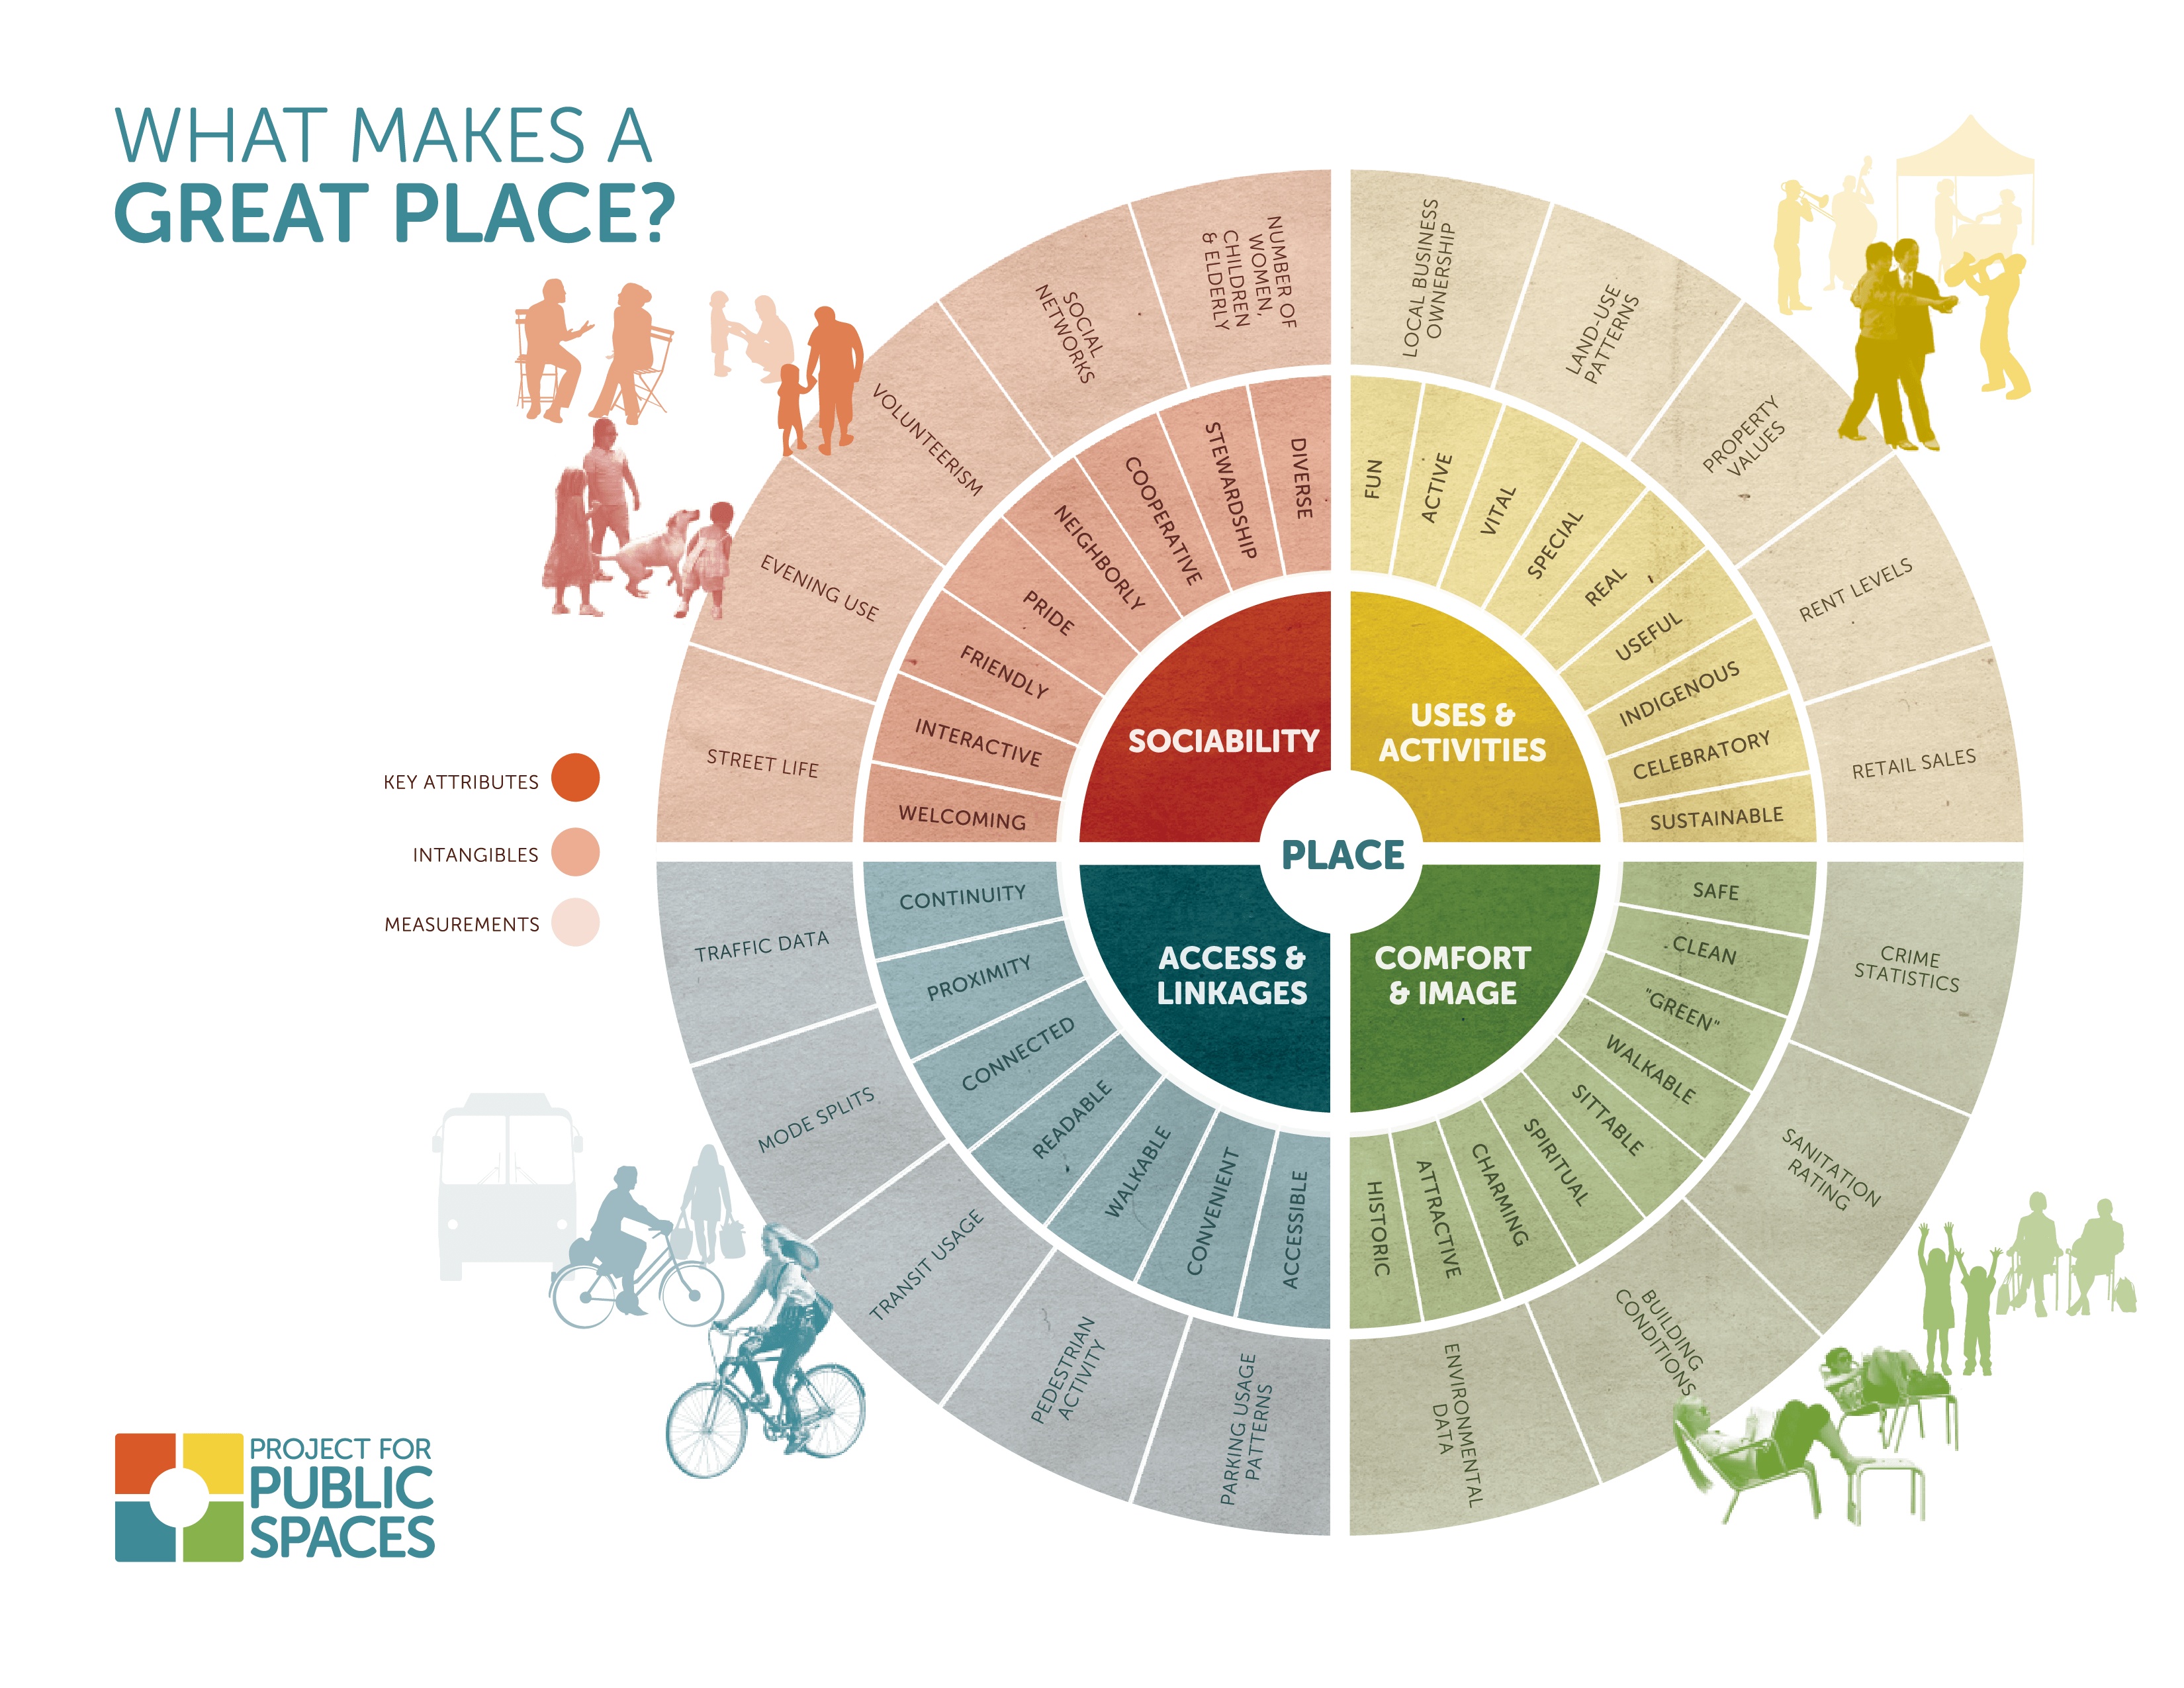
\includegraphics[width=10cm]{Illustrations/great_place.png}
\caption [What makes a great place?] {The four key attributes in the centre are surrounded by the intangibles and the indicator through which one can measure quality of the key attributes.}
\label{great_place}
\end{figure}
%%%%%%%%%%%%%%%%%%%%%%%%%%%%%

Around the same time in architectural research Bill Hillier developed his theory of what he called \textit{Space Syntax}. He generalised that cities need to be considered as an arrangement of architectural layouts that are defined through their relationships between physical space and social life reflected in movement patterns and activities of its inhabitants \cite{Hillier_1989}. 
To put it differently, \textit{Space Syntax} \index{Space Syntax} aims to analyse the spatial morphology of cities through researching the "relation of space to society, [which] is mediated by spatial configuration. Spatial configuration proposes a theory in which we find pattern effects from space to people and from people to space" \cite{Hillier1998}. This architectural theory as been applied and proofed in the fields of urban design (reference), architecture (reference), but also in cognitive science (Dalton et al., 2006) and in design and development of pervasive systems (Kostakos et al., 2009) and in particular in public displays (Dalton et al. 2010). In the meanwhile a methodological tool-set provided by Space Syntax facilitates the systematic study through spatial analysis and empirical observations of human behaviour such as pedestrian movement or social encounter in the urban realm \cite{AlSayed2013}.

%Dalton, R. C., Hölscher, C., & Turner, A. (2006). Space syntax and spatial cognition. Space Syntax and Spatial Cognition, (September), 1–201. https://doi.org/10.1177/0013916502238864
%Kostakos, V. (2009). Space Syntax and Pervasive Systems.
%Dalton, S. N., Marshall, P., & Dalton, R. C. (2010). Measuring environments for public displays. Proceedings of the 28th of the International Conference Extended Abstracts on Human Factors in Computing Systems - CHI EA ’10, 3841. https://doi.org/10.1145/1753846.1754066

The theoretical foundation of this research includes the description of the triangular relationship between a given Spatial Layout, the Attractor and Movement (fig. 2).
%Hillier, B. et al., 1993. Natural Movement: or, configuration and attraction in urban pedestrian movement. Environ Plann B. Available at: http://eprints.ucl.ac.uk/1398 [Accessed December 1, 2013].

%%%%%%%%%%%%%%%%%%%%%%%%%%%%%%%%

\begin{figure}[h!] 
\centering
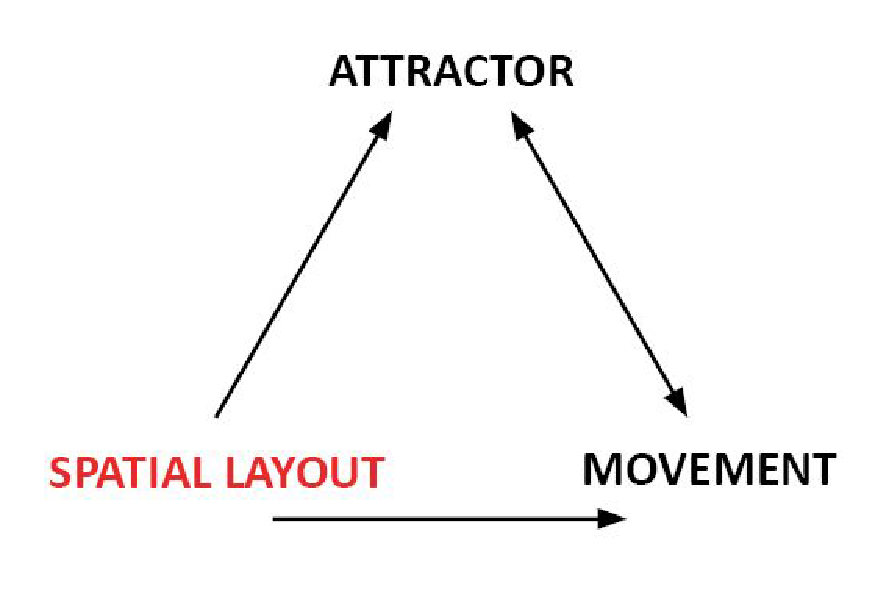
\includegraphics[width=6cm]{Illustrations/attractor_movement.pdf}
\caption [Spatial Layout, Attractor, Movement] {Socio-spatial configuration of public space: spatial layout, attractor and movement according to Hillier et al. (1993).}
\label{attractor_movement}
\end{figure}
\smalltodo[size=\footnotesize]{3D line drawing of an urban situation where the Spatial Layout has red lines, the attractor (i.e. a media facade) is blue and people within are marked green to illustrate the abstract sketch.}

%%%%%%%%%%%%%%%%%%%%%%%%%%%%%%%%

The arrangement of solid building blocks and the void space around it form the Spatial Layout \index{Spatial Layout}. Spatial layouts differ in their function and usage. Hence a central pedestrianised square differs from a traffic congested linear high street. 
Various Patterns of spatial layouts have been studied by Alexander (reference) and Lynch (reference).

\textit{Attractors}\index{Attractors} are physical objects which can be of different scale arranged  within the Spatial Layout that draw people's attention or entice people to step out of their daily routine. On a small scale attractors can be street furniture such as benches, ping-pong tables or water fountains, on a medium scale one can mention cafes, restaurants, bars and shops, whereas on a larger scale it could be historical facades, architectural landmarks or media facades. In this dissertation I consider large electronic surfaces such as urban screens or media facades as attractors. Besides their physical and spatial properties attractors have temporal qualities as well. For instance during rain one might avoid sitting on an outdoor bench and prefers to sit in a cosy bar, whereas during a warm summer afternoon people choose to enjoy cold beverages whilst sitting in front of a bar watching other people's activities.

Movement\index{Movement} is a major component in the formation of public space.
Seamon defines movement as "any spatial displacement of the body or bodily parts initiated by the person himself or herself" (Seamon, p.53). 
He further argues that the body and its extension in space and time are the essential components for an experience. Out of a sequence of movements and gestures evolves the ‘body ballet’ (Seamon, p.54). 
As soon as we locate the ‘body ballet’ into a specific physical environment we create the ‘place ballet’.
The type of movement - i.e. standing, strolling, rushing, running
Movement also has to do with people's attitudes. For example they rush to work in the morning whereas in the evenings they wander aimless through the city getting excited by different attractors.
The type of spatial layout and attractors within impact our movement. Transit spaces where people rush in order to catch a bus are different to public parks where people gather for pick-nicks.



A visible example of the triangular relationship described above is given by Jacobs:
Liveable streets in small scale neighbourhoods are the places where people meet and where commercial activities animated by cafes, restaurants, bars, bakeries and book stores take place. 
People love watching activities on the side walk generated by ordinary people, who run their daily errands (Jacobs). 
Jacobs wrote about primary children, who “dribble” to school, business men and elegant women heading for public transport and women in house dresses “criss-crossing with one another” and stopping for short conversations (Jacobs, 1961: 66-67). Jacobs identified this order of movements as a sidewalk ballet.
Not in a strict definition as a sequence of steps and movements in dance following a written notation but rather in a random alignment of improvisation of movements with ongoing new situations which demand human interactions (Jacobs, 1961: 65). 
At the same time one has to understand that the social activities in a public space change during the course of a day and even throughout the year.   
This is a glimpse on the strong spatio-temporal relation urban street life comprises. 


%‘Embodied interaction’ (Dourish, 2001), which describes action of the 'body' or user interacting with embedded technology (and thus potentially linking to social networks) is another important component in location-based applications

The given Spatial Layout, Movement and Attractors are interdependent key properties of what I will call in this dissertation \textit{socio-spatial configurations}. It is to notice that a given Spatial Layout may impact the configuration of Attractors and Movement. Attractors and Movement do influence each other, whereas neither of the both have an impact on the Spatial Layout 


\paragraph{The Digital Shift}

At the same time the city undergone a radical shift widely invisible and hidden from most citizens. The 'invisble city' (Lewis Mumford) 


In the meanwhile: 

%%%%%%%%%%%%%%%%%%%%%%%%%%%%%%%%

\begin{singlespace}
	\leftskip2.3em
		\rightskip\leftskip
			\textit{\small The visible city as a prime determinant of the urban is an artifact of the past. Instead, it is what Lewis Mumford called the "invisible city," the world of cables, wires, connections, codes, agreements, and capital that increasingly dominates our networked society [Lewis Mumford]. We stand at the dawn of the regime of the invisible, its role in determining urban structure vast. The visible becomes an irruption of other forces, a graphic user interface for a more powerful command line below [Varnelis].}
\end{singlespace}

%%%%%%%%%%%%%%%%%%%%%%%%%%%%%%%%

Based on Mamford Kittler concluded that the City as a Medium (Kittler, 1996)
 
%Thus she set up four conditions to improve street life. 
%First, she claims for street activities at all hours of the day. 
%Neighbourhoods have to attract all kinds of different people. 
%This is attainable through a mixture of uses and functions, both socially and economically. (Jacobs, 1961: 198-232) 
%Her second condition is the building of short blocks and intricate street structures which provides the possibility for pedestrians to explore different walks (Jacobs, 1961: 233-243). 
%Variation of buildings in age and function is the third condition for successful street life (Jacobs, 1961: 244-260). 
%The last one is density, because the higher the concentration of people in one place is the more attractive the area. 
%Neighbourhoods with working vivid street life determine safety, social cohesion and economic growth is Jacobs' conclusion (Jacobs, 1961: 261-289).
%To summarize, one can say that Jacobs' criticism of the prevailing architectural styles and urban planning ideologies and her persistent observations on \textit{life in between buildings} (book title by Jan Gehl) initiated a shift from form-follows-function towards a behavioural centric age.  

%With the advent of the digital our built environment has turned into an ecology of sensors measuring our behaviour in public. Human-computer interfaces such as mobile devices, urban screens or media facades augment our physical presence in digital space. 

%%%%%%%%%%%%%%%%%%%%%%%%%%%%%
In summary: Whilst modernist architects (references) focused on the physical properties of humans Jacobs and others (Seamon, Goffman, ...) explored human behaviour in relation to public space. 
Jan Gehl later accused this architectural period of lacking the people scale, which needs to work on eye-level and 5km/h perception, which in a nutshell was the method Jacobs applied in her observations. Whilst architects persistently neglected the importance of public spaces for creating social interactions Jan Gehl was one of the pioneers who put the results of his research into practice \cite{Gehl_2013}. 

To summarise 
I briefly summarised the notion of public space .
In this section I defined what I consider spatial configuration, namely the triangular relationship between Spatial Layout, Movement and Attractors. 
what I consider the notion of public space with regards to this research is: 
Firstly public space is constituted through the three components of Spatial Layout, Movement and Attractors. 
Guidelines on how to approach public spaces when designing for interactions include:
The people scale as suggested by Gehl.
Some of the conditions Jacobs suggested:
Street activities need to take place during all hours of the day. I would argue that this increasingly includes the hours of night. Further a mixture of uses and functions, both socially and economically. 
Designing for density, the more people there are in one place the more attractive this area is - of course overcrowding leads to the opposite. 

In the next section I will investigate what interactions are and how technology may assist in mediating those interactions in public space.


%%%%%%%%%%%%%%%%%%%%%%%%%%%%%

\section{Shared Encounters and Technology Mediated Interactions in Public Spaces}

Only recently digital technologies entered the public domain in form of mobile devices or large situated electronic surfaces and discussions are ongoing whether digital technologies affect social interactions in public space have adverse effects \cite{Turkle_2012}, have no impact \cite{Hampton_2015} or can be seen as an opportunity to create mediated participatory experiences \cite{Gordon_2011}. Hence the key concept of \textit{Public Space} and the triangular relationship between Spatial Layout, Attractor and Movement is followed by a review of research into what constitutes a shared encounter and how it differs from an interaction in public space.

Encounters are different in their nature and are situated either in private or in public spaces. They are individual or grouped and either they are planned or happen by chance. The characteristics of shared encounters have been characterised by Willis et al. (2010) as:

%%%%%%%%%%%%%%%%%%%%%%%%%%%%%%%%%

\begin{singlespace}
	\leftskip2.3em
		\rightskip\leftskip
\textit{\small the interaction between two people or within a group where a sense of performative co-presence is experienced and which is characterised by a mutual recognition of spatial or social proximity} 

\small Taken from  Willis et al. (2010) p.4
\end{singlespace}

%%%%%%%%%%%%%%%%%%%%%%%%%%%%%%%%%
Today, as ICTs are ubiquitous and mobile, people interacting with each other does not require them to be in the same physical space any more, instead we create co-presence where two people interact with each other without being in the same physically space. Hence the encounter is technology mediated and therefore defined as a shared encounter.
Social spaces are defined as a series of interactions and their nature is volatile - movement.

%Willis: "our interactions with other can be considered as situated in that they are shaped by both the physical setting and the social situation - consequently we behave differently in different situations"
%Willis: "Social spaces emerge through multiple one-to-one interactions and by participation in groups. These encounter spaces can disperse as rapidly as they are created, but some can become more established and exist for a period of time."
Goffman (reference) describes the part performance plays in an interaction; performances are a set of activities of an individual before a set of observers - either friends of strangers

Social encounters are defined as unplanned ad-hoc gatherings amongst (un-) known people. Research has defined ‘shared encounters’ as mostly context aware. The physical setting in which an encounter takes place is relevant (Goffman, 1963), hence the "built environment creates stages for shared encounters but sometimes the features of built space can actually hinder rather that allow these shared experiences" (Garcia). Therefore the type of encounter stage and its information context impacts the kind of shared encounters. Encounter stages are public spaces “on which people negotiate boundaries of a social and cultural nature” (Fatah et al, 2005). For example at bus stops social chance encounter happen when people ask for directions or start conversations about the delayed schedule. One objective of this research will focus on the particular spatial properties physical encounter stages require in order to support shared encounters.
\smalltodo[size=\footnotesize]{This argument can be confirmed in my findings of the case studies - e.g. participants in Sao Paulo and Linz were discussing the impact of public visualisations. }

 

(Willis, Shared encounters)).
Fatah defines three different types of encounters Fig. \ref{DigitalEncounterFatah}). 
and consequently a "concept of a digital stage that can facilitate and encourage different types of social encounters" has been developed. 

%%%%%%%%%%%%%%%%%%%%%%%%%%%%%

\begin{figure}[h!] 
\centering
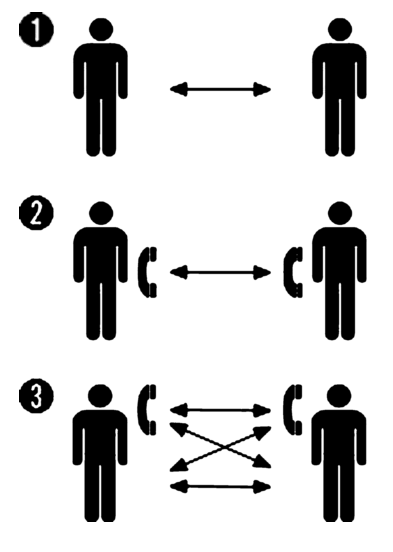
\includegraphics[width=3cm]{Illustrations/DigitalEncounterFatah.png}
\caption [Digital Encounter Fatah] {Digital Encounters: Human communication (1), communication replaced by technology (2), or augmented by technology (3).}
\label{DigitalEncounterFatah}
\end{figure}

%%%%%%%%%%%%%%%%%%%%%%%%%%%%%

To summaries: 

- need to build in ‘familiar stranger’ (Milgram 1977)

\subsection{Urban Interaction Design - Urban IxD}

%%%%%%%%%%%%%%%%%%%%%%%%%%%%%

Interaction Design (IxD) is a relatively new discipline that merges design with digital technologies and behavioural science and hence founded on divers academic and applied fields (Fig. \ref{DesignFields}).
IxD is about creating interactive products for the user experience to "enhance and augment the way people work, communicate and interact" (\cite{Rogers_2015} p.9).
Research into Human-Computer Interaction (HCI) has spawned Interaction Design \cite{Rogers_2015} to better understand "wicked problems" (Rittle and Webber, 1973; Fitzgerald, 2003; Zimmermann, 2007) created through sometimes unpredictable human behaviour.
%Rittel, H.W.J. & Webber, M.M., 1973. Dilemmas in a general theory of planning. Policy Sciences, 4(2), pp.155–169.

%%%%%%%%%%%%%%%%%%%%%%%%%%%%%

  \begin{figure}[h!]
  \centering
  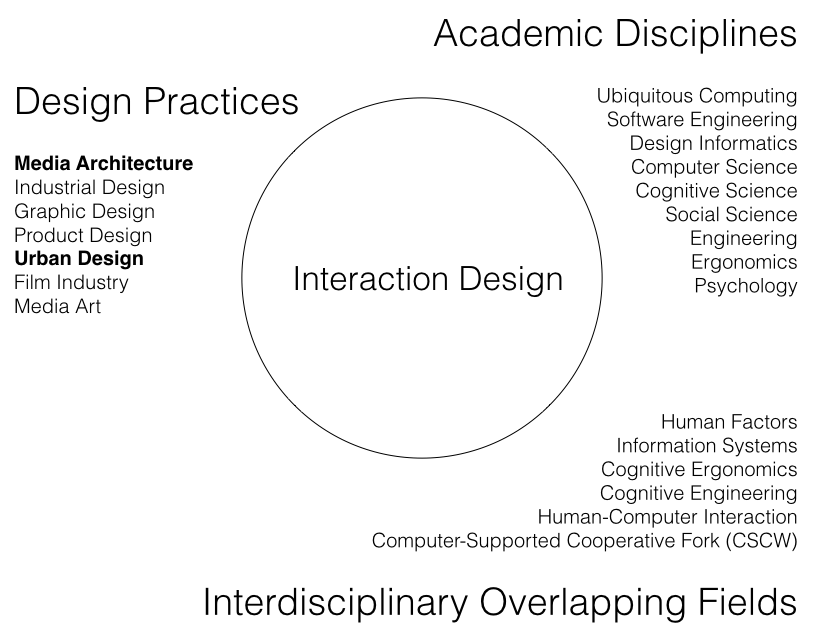
\includegraphics[width=8cm]{Illustrations/Interaction-Design-Fields.png}
  \caption{What is Interaction Design? \cite{Rogers Interaction Design - beyond HCI 4th Edition p. 9} - What is missing here is the overlapping of interaction design and media architecture.}
  \label{DesignFields}
  \end{figure}

%%%%%%%%%%%%%%%%%%%%%%%%%%%%%
The invention of the computer mouse by Engelbart in 1963 might be seen as the first IxD product as it incorporates knowledge from design, behavioural science and computer technologies.   
Apple's iPod in turb can be considered as one of the first commercial IxD products with global success that follows clear IxDs principles (Moggridge, 2006). Here the touch interface and the required gestures to use the portable music player is pioneering IxD. 
%Moggridge, B., 2006. Designing interactions - Chapter 1, Available at: http://site.ebrary.com/lib/aalborguniv/reader.action?docID=10173639.

IxD mostly develops screen-based applications and services for desktop computers or more recently for mobile devices such as smart phones or tablets. However, since the advent of ubiquitous computing (Weiser, 1991), and its application in urban space in the form of urban computing (Kindberg et al., 2007), the built environment incorporates architecture and ubiquitous computing technologies. Consequently IxD entered the urban domain and began to design way finding or location based applications that let user experience services such as bike or car sharing in new ways.
%The Internet of Things (IoT) is another application worth mentioning in this context.

In academia the research project "Digital Urban Living" at the Aarhus University was the first larger attempt to explore IxD in an urban context \footnote{http://digitalurbanliving.projects.cavi.au.dk/ accessed 29.11.2016} Within this project researchers and designers in collaboration with the CAVI centre \footnote{http://cavi.au.dk/about-cavi/ accessed 29.11.2016} implemented amongst others "Aarhus by Light" \footnote{http://cavi.au.dk/research-areas/aarhus-by-light/ accessed 29.11.2016} media facade project at the Concert Hall in Aarhus (Brynskov et al., 2009) that explored interactive systems for user engagement in urban space.
%Brynskov, M. et al., 2009. Staging urban interactions with media facades. In Lecture Notes in Computer Science (including subseries Lecture Notes in Artificial Intelligence and Lecture Notes in Bioinformatics). pp. 154–167.

%%%%%%%%%%%%%%%%%%%%%%%%%%%%%%%
\begin{figure}[h!]
  \centering
  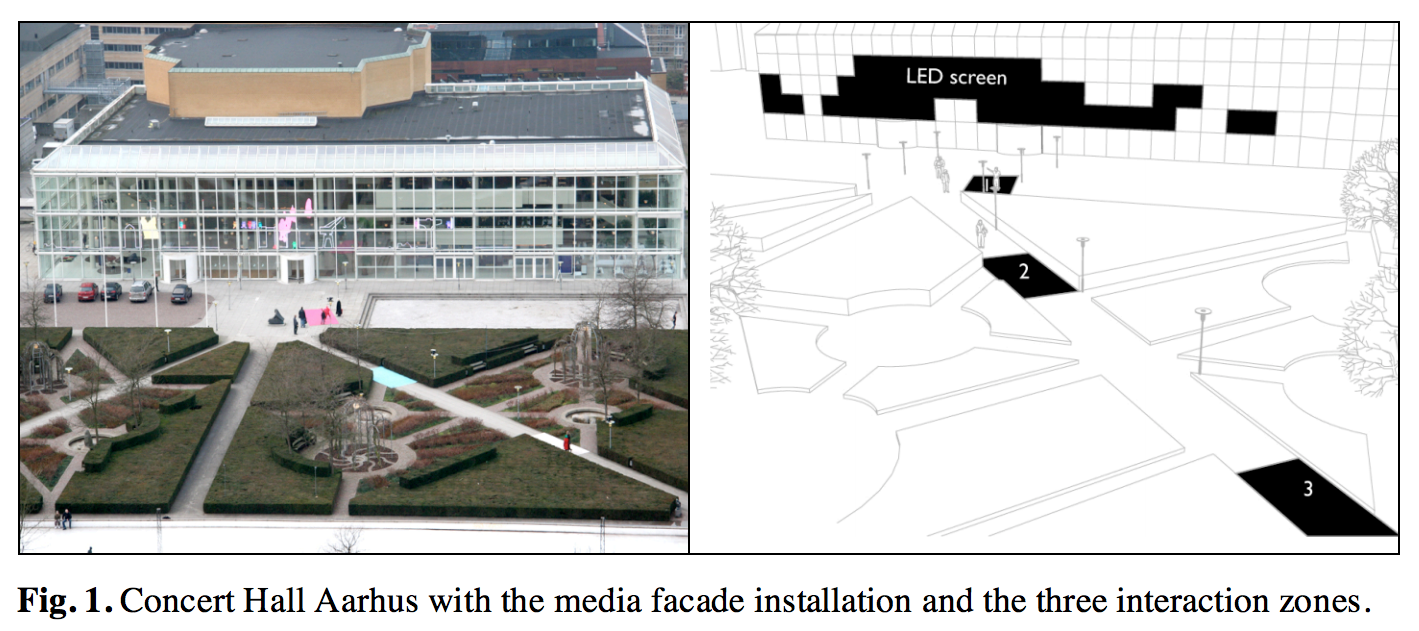
\includegraphics[width=14cm]{Illustrations/AarhusbyLight.png}
  \caption{Aarhus by Light}
  \label{AarhusbyLight}
  \end{figure}
%%%%%%%%%%%%%%%%%%%%%%%%%%%%%%%

From the spatial perspective (which will be discussed in detail later in this backround research) urban IxD benefited from Fischer's and Hornecker's research into an understanding of interaction spaces in public spaces \cite{Fischer_2012}.
Whilst designing for interactions mediated by interactive technology in public spaces has been predominately occupied by HCI and IxD there are academic initiatives and projects from architectural research and practice (Behrens, 2013).
%Behrens, M. (2013). Exploring the effect of spatial layout on mediated urban interactions. Proceedings of the 2nd …. Retrieved from http://dl.acm.org/citation.cfm?id=2491586

- Screens in the Wild
- 


Early social implications of interactive systems on urban grassroots movements have been explored by the HCI community during a CHI \footnote{ACM Conference on Human Factors in Computing Systems (CHI)} workshop in 2011 by (Kuznetsov et al., 2011).
%Kuznetsov, S., Odom, W., Paulos, E., Disalvo, C., Moulder, V., Wakkary, R., & Hirsch, T. (2011). HCI , Politics and the City : Engaging with Urban Grassroots Movements for Reflection and Action. Design, 2409–2412. http://doi.org/10.1145/1979742.1979568

The social aspects in urban IxD are currently explored in the European wide network called OrganiCity. The approach is to provide "cooperation and participation, for collaborative city experiments developed with, and at the initiative of, citizen groups, organisations, authorities and companies." In several projects across European cities the advancement of participatory city making mediated by digital technologies and IxD are investigated.  \footnote{The EU funded OrganiCity initiative connects leading smart cities Aarhus, London and Santander with the aim to "put people at the centre of the development of future cities." http://organicity.eu/ accessed 25.11.2016}

Urban IxD and wellbeing have been explored by  

%usability goals for a sustainable user experience which are: the effectiveness of use (how good is a product at performing as it should do?), the efficiency of use (Is the device able to sustain a high level of productivity?), the safety of use, the utility (Does the product provide an appropriate set of functions that will enable users to carry out their tasks in the way they want to do them?), the ease of learning (Is it possible to work out how to use the product by exploring the interface and trying out certain actions?) and the memorability of usability (What kind of interface support has been provided to help users remember how to carry out tasks?).

Research into IxD has brought forward several frameworks for designing interactions in urban space.
- technical aspects
-social aspects
- spatial aspects Daalsgarqd, Halskov ... 
From behavioural perspective designing for interactive products the following principles have been established by : "1) Affordance: This term refers to the question How easy is it to find out how to use it?. Thus a physical object has to explain itself in relation to how to use it by its obvious perceptional appearance. (Norman, 1988). 
2)Visibility: Controlling devices such as buttons basically have a very clear visibility. But far more important is the positioning of a device in the environment. If people cannot find the device, there will be no interaction (Rogers, 2011).
3) Accessibility: An interactive device has to be accessible by as many people as possible. Especially nowadays where technical progress is accelerating the integration of as many groups of people as possible this is an important aspect in interaction design. (Rogers, 2011; Negroponte, 1995)
and finally 4) Feedback: An immediate feedback such a flashing light or audio signal by the device is a crucial element to let the user know that the interaction works (Rogers, 2011)."	



These requirements are therefore integral part of the development of our project. 

%In the context of interaction design around public displays in an urban context the following research projects can be aligned:
%Elmar Trefz and Joanne Jakovich: Rapid Probing: Setting out methods and a framework for Urban Interaction Design - Media City 4
%- Urban IxD projects in research:
%1. Community notice board Sydney
%2. MyPosition
%3. Lisa Koeman, V Kalnikaite, Yvonne Rogers, Jon Bird	What chalk and tape can tell us: Lessons learnt for next generation urban displays	2014	PerDis 2014 - Proceedings: 3rd ACM International Symposium on Pervasive Displays 2014, Journal article

In summary: Designing means knowing your limitations and constraints. This is a finding that applies to architectural designing and IxD designing for interactions. 
This thinking applies for research as well.

%%%%%%%%%%%%%%%%%%%%%%%%%%%%%%%

\begin{singlespace}
	\leftskip2.3em
		\rightskip\leftskip
\textit{\small Good design comes from the successful synthesis of a solution that recognises all the relevant constraints, and the nature of the constraints defines the difference between the design disciplines.} 

\small Taken from Moggridge (2006) p.649.
\end{singlespace}

%%%%%%%%%%%%%%%%%%%%%%%%%%%%%%%

\subsection {City as Interface}

For some people to be able to encounter new people or to interact with each other without being in the same physical space interfaces that mediate communication may assist.
Today such interfaces are ubiquitous, we seem to have established an "interface culture" (Johnson, 1997) 
%Interface Culture: How New Technology Transforms the Way We Create and Communicate)
in which individual mobile devices or shared and situated large electronic surfaces structure our everyday lives (Saggio,).
However definitions of what interfaces in public spaces actually constitute are blurry and due to their interdisciplinary usage manifold.  

Going back to the early considerations in computer science, Yershov suggested the properties needed for a "dialogue between man and machine" (Yershov,). In his understanding an interface has to be "conform to the characteristics of interpersonal communication, since these are rooted in the characteristics of human intelligence."
Nevertheless the user needs to train himself to be able to communicate with the machine. 
This finding complements the notion of digital encounters as described in the previous section.
Interpersonal communication has been studied by Norman (1988).
%Norman, D. (1988) The Design of Everyday Things.
%Goffman, E.: Behaviour in Public Places. The Free Press, New York (1966)
%There is even a whole new profession of so called interface designers.

%%%%%%%%%%%%%%%%%%%%%%%%%%%%%%%

\begin{figure}[h!] 
\centering
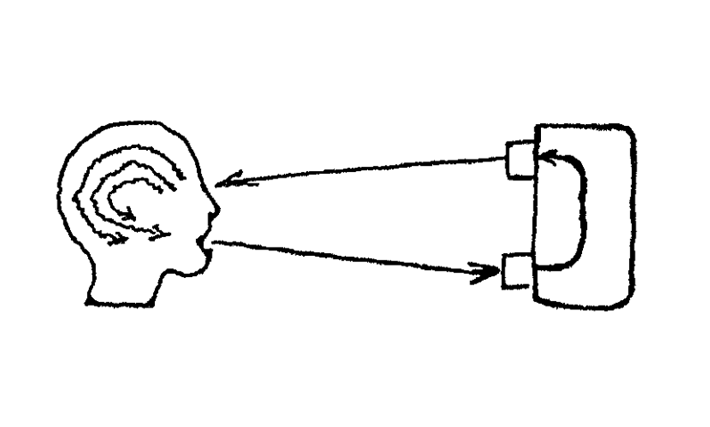
\includegraphics[width=8cm]{Illustrations/Yershov.png}
\caption [Director-agent interaction diagram by Yershov (1965)] {"The machine above all as a means of automating the mental activities of man, or as - this term seems more appropriate - an amplifier of the mental abilities of man" (Yershov, 1965). Negroponte (1970) commented, that the three arrows within the human brain compared to the single arrow within the machine would imply "an ever-continuing act particular to the role or constitution of the man and not the machine."}
%“The Architecture Machine” by Nicholas Negroponte (published by the MIT in 1970). 
\label{Yershov}
\end{figure}

%%%%%%%%%%%%%%%%%%%%%%%%%%%%%%%
These early considerations of how humans interface computers has led to the research domain called human-computer interaction.
One is aware of the early interfaces that emerged during the what is called "2nd wave" of HCI, when Tangible User Interfaces (TUIs) such as the mouse and keyboard together with Graphical User Interface (GUI) gave access to yet bulky computers. 

While it has been claimed that so called Graphical User Interfaces (GUI) are the most widely spread products of HCI that allow humans to interface with computers,  Tangible user interfaces (TUIs) "give physical form to digital information, employing physical artifacts both as representations and controls for computational media" \cite{Ullmer_2000}(p. 916). 
\textit{Tangible Interactions} evolved from research in TUI and rely on embodied interaction, tangible manipulation, physical representation of data and embeddedness in real space and give computational resources and data material form \cite{Hornecker_2006}. 

Others argue that the shift from situated (i.e desktop computer) to mobile interface (i.e. mobile phones or tablets) and its ubiquitous use in public space blurs the boundaries between the physical and the digital social networks and hence interfaces can be described as 'social interfaces'(de Souza e Silva, 2006).  

%%%%%%%%%%%%%%%%%%%%%%%%%%

\begin{singlespace}
	\leftskip2.3em
		\rightskip\leftskip
\textit{\small I propose a further conceptualization of “social interface,” which defines a digital device that intermediates relationships between two or more users. Within this context, social interfaces not only reshape communication relationships but also reshape the space in which this interaction takes place.} 

\small Taken from de Souza e Silva, A. (2007) p.261-262
\end{singlespace}

%%%%%%%%%%%%%%%%%%%%%%%%%%
%de Souza e Silva, A. (2007). From cyber to hybrid: Mobile technologies as interfaces of hybrid spaces. In D. Bell & B. Kennedy (Eds.). The Cybercultures Reader 2.0 (pp. 757-772). London, New York: Routledge. (re-print from Space and Culture journal).
And beyond the social component de Souza e Silva refers to the impact social interfaces ultimately have on the space in which they take place. This is in line with the notion of encounter stages. 

Hookway understands interfaces as a "relation with technology" rather than a technology in itself (Hookway, 2014).

%%%%%%%%%%%%%%%%%%%%%%%%%%

\begin{singlespace}
	\leftskip2.3em
		\rightskip\leftskip
\textit{\small The interface is a form of relation that obtains between two or more distinct entities, conditions, or states such that it only comes into being as these distinct entities enter into an active relation with one another; such that it actively maintains, polices, and draws on the separation that renders these entities as distinct at the same time as it selectively allows a transmission or communication of force or information from one entity to the other; and such that its overall activity brings about the production of a unified condition or system that is mutually defined through the regulated and specified interrelations of these distinct entities.} 

\small Taken from Hookway, B., 2014. Interface, p. 4
\end{singlespace}

%%%%%%%%%%%%%%%%%%%%%%%%%%
And for Galloway "interfaces are not simply objects or boundary points. They are autonomous zones of activity. Interfaces are not things, but rather processes that effect a result of whatever kind."
According to Galloway's notion of Interfaces defines "Activity zones", which is in support of the idea of social encounter stages as defined by (ref.) 
Verhoeff (reference) finally summarises that: "Following Branden Hookway and Alexander Galloway, I understand media interfaces as processes rather than objects. An interface is not something; it does something."
%Urban Interfaces: The Cartographies of Screen-Based Installations by Nanna Verhoeff (2016)
%Due to technological advancement, large public displays became ever more incorporated into the built environment and because of price decline its application for social and artistic purposes became popular in urban space. 
%This led to novel technology-mediated social interactions, such as people engaging with media facades through tangible devices.


Seen from architectural research Martyn Dade-Robertson (2013) introduces Architectural User Interfaces (AUIs) taking into account Graphical User Interfaces (GUIs) and argues that architectural design and HCI can benefit immensely from each others.
Dade-Robertson refers to McCullough (2004) who back then saw:

\begin{singlespace}
	\leftskip2.3em
		\rightskip\leftskip
\textit{\small Digital networks are no longer separated from architecture. Unlike cyberspace, which was conceived as a tabula rasa, pervasive computing has to be inscribed into the social and envirnonmental complexity of the existing physical environment.} 

\small Taken from Malcom McCullough, 2004. Digital Ground, page 4.
\end{singlespace}

Dade-Robertson concludes that the future of architectural design is accompanied by cognitive science and situated and pervasive interfaces.
%McCullough, Malcom, 2004, Digital Ground: Architecture, Pervasive Computing and Environmental Knowing, MIT Press
%(Dade-Robertson, M. (2013). Architectural User Interfaces: Themes, Trends and Directions in the Evolution of Architectural Design and Human Computer Interaction. International J of Architectural Computing, 11(1), 1-19.)

Martijn de Waal even extends the notion of an interface and considers the whole city as an interface.

%de Waal, M., 2014. The City as Interface - How Digital Media are Changing the City.

One of the first large scale social media art projects that provided an interface allowing passers-by to create and share content on a media façade was the BlinkenLights \footnote{http://blinkenlights.net/blinkenlights accessed 28.11.2016} project in 2001. Participants on a street in Berlin were able to share messages typed into a mobile phone with the public through posting them on a low-resolution media facade (each pixel was represented through an illuminated window in an office building (i.e. Haus des Lehrers, Alexander Platz, Berlin)). 
Since then numerous media art and research projects have been developed and presented that include user interfaces and applications to transmit actions, in situ and in real-time, on to a media facade that is connected to an interface. 
For example, SMSlingshot \cite{Fischer_2012}, Sonic Skate Plaza \cite{Serret_2013} or Binoculars \cite{Guljajeva_2013}.
In applied HCI research, more recently, multi-user interactions with media facades through mobile devices revealed challenges when deploying interactive artifacts in urban space that enable passers-by to engage with media facades \cite{Boring2011}. 
Wiethoff and Gehring \cite{Wiethoff2012} introduced a design toolkit to prototype when designing interactions with media facades before the actual deployment. 
\index{In-the-air-tonight} A media facade project that explored mobile interfaces to rise awareness of social issues in Toronto has been developed by the Ryerson Image Centre. During winters night the LED facade is turned in blue to represent the wind speed, as soon as the hashtag \#homelessness appears on Twitter the building's facade flashes up in red light \footnote{http://www.intheairtonight.org/ accessed 28.11.2016}. 

Since then, novel interfaces have been designed and deployed in the urban environment that let people interact with media facades \cite{Hoggenmueller_2014}.

%Fischer, P.T.; Hornecker, E., 2017. Creating Shared Encounters Through Fixed and Movable Interfaces. , pp.163–185. Available at: http://link.springer.com/10.1007/978-981-10-1962-3.

In summary: HCI considers interfaces as pure physical or graphical representations that allow users to access computer technologies. Today different disciplines understand that interfaces unfold temporal, social, spatial and cultural dimensions and designing interfaces can not neglect these dimensions.
What does it mean when one aims to design for interactions with media architectures?



%%%%%%%%%%%%%%%%%%%%%%%%%%%%%

\subsection{Communication Technologies for Mediated Encounters}

WiFi
Bluetooth
RFID

%%%%%%%%%%%%%%%%%%%%%%%%%%%%%

\subsection{Public Display Research}

Long before research into public displays \index{public displays} became a domain within HCI, various kinds of electronic displays and digital signage appeared in public spaces.
At the New York Times building the first public display, \textit{The Motogram} \index{The Motogram (Zipper)} also called \textit{The Zipper}, was installed in 1928 (Fig.\ref{DigitalSignage} (left)). The novel display consisted of a band of light bulbs (dot matrix\footnote{two-dimensional array of programmable objects, in context of this dissertation the objects are light- bulbs or LEDs}) that circulate breaking news along the facade. 
Almost fifty years later, in 1976, the same building got upgraded with the first large programmable electronic surface called \textit{Spectacolor Board} \index{Spectacolor Board}(Fig.\ref{DigitalSignage} (right)).
The rather conventional rectangular screen was mounted to the slim front side of the corner building facing towards Times Square; unlike \textit{The Motogram's} slim horizontal luminous strip which ran across all sides of the publishing house visually separating the building in a lower and an upper part. 
From an architectural point of view the analogue light bulb display conforms the architecture of the building through adapting to the characteristics of the facade. Whereas the \textit{Spectacolor Board} appears to be an oversized TV screen - attached to a wall that is too little. However, the \textit{Spectacolor Board} provides more opportunities for content creation as well the direction it is facing towards (i.e. Times Square) is very likely to reach a larger audience. Whilst \textit{The Motogram} due to its elongated shape is limited in content and can hence only show continuous running text it is specifically designed for the news agency New York Times.
Consequently, I argue that \textit{The Motogram} can be considered to be architectural compared to the \textit{Spectacolor Board}, which constitutes a public display in the form of an Urban Screen instead.

%%%%%%%%%%%%%%%%%%%%%%

\begin{figure} [h!]
    \centering
        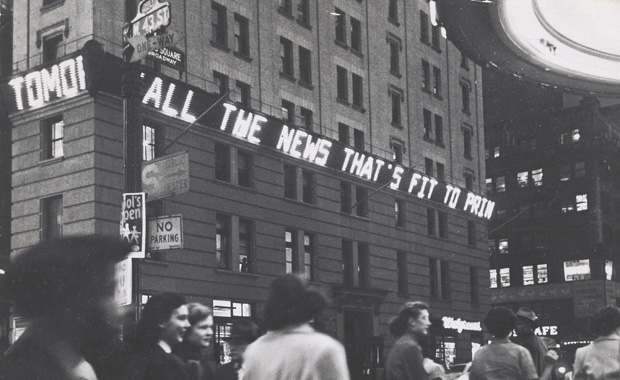
\includegraphics[height=4.5cm]{Illustrations/zipper.jpg}
        	%\caption[a]{Urban Screen}
      	%\label{UrbanScreen}
        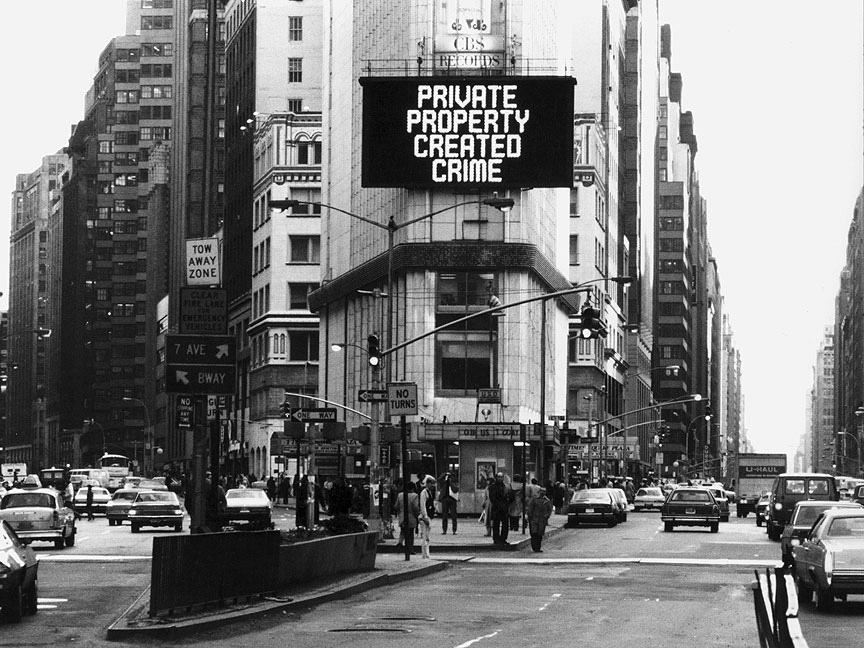
\includegraphics[height=4.5cm]{Illustrations/Spectacolor_JennyHolzer_.jpg}
       		%\caption[b]{Media Facade}
       	%\label{MediaFacade}
    \caption[First public displays]{Innovativ public displays at the New York Times Square: \textit{The Motogram/Zipper} display (left), and the \textit{Spectacolor Board} (right)}
    \label{DigitalSignage}
\end{figure}

%%%%%%%%%%%%%%%%%%%%%%

In the meanwhile public displays \index{public displays} are everywhere - mostly for commercial or informational purposes. Large screens at traffic junctions dazzle car drivers with dynamic advertising and at bus and train stations or airports huge displays update us on the latest travel news.  

Research in public displays \index{public displays} arose as observations by HCI researchers hinted towards different kind of human behaviour when having a home display in a public space for shared purposes. 
(Mention Rogers in the Wild?)
Although utility, usability and likeability seemed to be identical it has been obvious that different requirement such as "public displays need to grab the attention of passers-by, motivate passers-by to interact with them, and deal with the issues of interaction in the public" (Mueller et al., 2010) 
%(Müller, J. et al., 2010. Requirements and design space for interactive public displays. In Proceedings of the international conference on Multimedia. pp. 1285–1294.)
This relates back to Movement.

\textbf{Different Form Factors}
Whilst most public displays have conventional formats to easily be able to show cross platform content, the form factors of some displays vary and yet "it’s difficult to say whether display walls, windows, magic mirrors, or something completely different will become a dominant form for digital signs, but it’s likely that use of digital displays will continue to increase dramatically." (Want and Schilit, 2012). 
%Want, R. & Schilit, B.N., 2012. Interactive digital signage. Computer, 45(5), pp.21–24.

(Show figure of Florian Alt's shape shifting study of the public display at Munich Airport.)

\textbf{Interactivity}
In this context interactivity ar  ound those displays becomes ever more important. In the meanwhile the audience - in particular children - expect digital signage to in corporate touch features \footnote{This is an observation we frequently made during field observations in the Screens-in-the-Wild project.}. 



I will specifically refer to research in public display here as methods have been well advanced and many studies were deployed particularly from the field of HCI and hence there is a lot we can learn in terms of designing for interactions with large electronic displays. 
Whilst for HCI researchers the novelty in this kind of researchers has been to leave the secure lab environment and to study in-the-wild (reference Rogers), for researchers and practitioners in architecture and urban design the advent of digital communication technology together with research methods into how to study mediated interactions opened up a new field of research and practice as well as a new material to design with.   

Extensive research has been conducted exploring the challenges when deploying public screens in urban space. 
The technical challenges of deploying display technology in urban space have been summarized in Lancaster (2). 
Mueller et all (3) explored how to attract passers-by to public displays and what it needs to notice interactivity. 

Soon networked interactions were explored. 
Some of which pretended to connect people between London and New York where \index{The Telectroscope (2008)} \textit{The Telectroscope} \footnote{A public artwork designed by artist Paul St. George near Tower Bridge in London in 2008. \url{http://www.artichoke.uk.com/events/the_telectroscope/} accessed 07.12.2016} served as a . Others called \textit{Hole in Space} by Galloway and Rabinowitz (1980) \index{Hole in Space (1980)} connecting New York and Los Angeles \footnote{}; \textit{Hole in the Earth} \index{Hole in the Earth (2001)} \footnote{\url{http://v2.nl/archive/works/hole-in-the-earth} accessed 07.12.2016} linking Rotterdam to Indonesia.
In a larger context through \index{Connecting Cities Network (CNN} \textit{Connecting Cities Network (CCN)} \footnote{"Connecting Cities is a European and worldwide expanding network aiming to build up a connected infrastructure of media facades, urban screens and projection sites to circulate artistic and social content. 
In opposition to the commercial use of these urban media, we establish them as platforms on which citizens can exchange – within the city as much as between cities.EU funded project Connecting Cities" \url{http://connectingcities.net/ accessed 07.12.2016}} interconnecting several European cities through an existing infrastructure of urban screens and media facades in public spaces.
One specific project that can be mentioned here as it has used a very specific display is \textit{Ready to Cloud} \footnote{\url{http://theconstitute.org/readytocloud/} accessed 07.12.2016} \index{Ready to Cloud}. 
A EPSRC funded research project into networked interfaces from an architectural perspective is the \textit{Screens in the Wild} \footnote{\url{https://www.bartlett.ucl.ac.uk/space-syntax/screens-in-the-wild}} \index{Screens in the Wild (2011)}.


The role of space, social proximity and full body performative interactions in shared urban spaces have been addressed (5). 

Awareness of the relevance of the Spatial Layout has been 
Through introducing ‘urban HCI’ \index{urban HCI} (6)the spatial aspects of urban media installations have been described. 
However, the background research presented has not addressed a number of highly significant aspects in particular the ones related to the dynamic nature of urban space (7) and their potential impact on the design of public displays. 

technical challenges of deploying display
technology in public space have been summarized by Streitz et al. (2003).

%%%%%%%%%%%%%%%%%%%%%%%%%%%%%

\section{Urban Media - From Electronic Surfaces to Media Architecture}

%Structure of this chapter:
%\begin{itemize}
%\item building projections
%\item public displays
%\item urban screens
%\item media facades
%\item media architecture
%\end{itemize}

%Structure of the typologies:
%\begin{itemize}
%\item definition and theory
%\item applied research and projects
%\item discussion focusing on components (technical), social and spatial aspects
%\end{itemize}

A medium is an information carrier for communications between different entities. Whilst traditional analogue media is considered to be print, audio or video related with the advent of digital technology and the world wide web there has been a shift towards screen based digital media called new media. 
An extended definition of what a medium is has been developed by McLuhan. According to him a medium not only transfers information but the components of the medium itself influence us.  
An intriguing example of a medium in the context of this dissertation is the light bulb. According to McLuhan the light bulb is a medium that brings people together at night and therefore "creates an environment by its mere presence." (McLuhan: Understanding Media, p. 8.)
Considering light bulbs including its newer version the LEDs as a material for electronic surface one can argue that media architecture as well creates such social environments.

about the term urban media "a text message enables us to reschedule a meeting at the last minute or send a quick personal message to a loved one in between all our activities; our smartphones enable us to conveniently look up information about our surroundings (‘where is the nearest café, restaurant, ATM?’); thanks to navigation systems, we reach our destinations more quickly, especially if the software is geared to receive live traffic updates and it can redirect us so we avoid traffic jams; mobile social networks such as Twitter and Facebook enable people to keep their ‘friends’ constantly informed about where they are, what they are doing and what they think of it all. These are all examples of urban media: a collective term that I use in this book for media technologies that in one way or another can influence the experience of a physical location." martijn de wal


The intention of the \textit{Fun Palace} \index{Fun Palace (1961)} (1961) by Cedric Price was  \index{Cedric Price} to design for a time-based, indeterminate, and anticipatory architecture.
The aim was to provide the user with time-based urban interventions and flexible or adaptable projects that invited the user’s participation (Fig.\ref{fun_palace}).
Hence the structure was quickly to assemble and taken apart when necessary.
Consequently the implications would trigger curiosities about unpredictable and incomplete worlds.

%%%%%%%%%%%%%%%%%%%%%%%%%%%%%

\begin{figure} [h!]
    \centering
        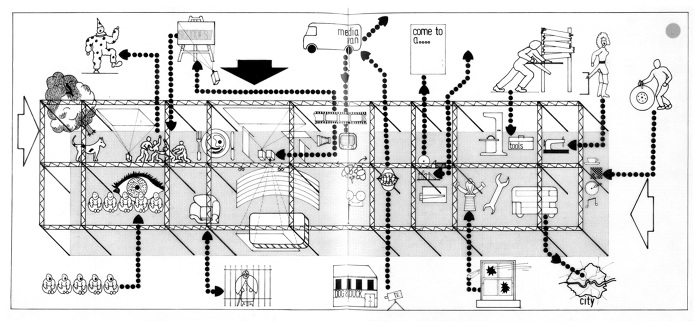
\includegraphics[width=\textwidth]{Illustrations/fun_palace.png}
    \caption[Fun Palace, (1961)]{Cedric Price's brainchild ... }
    \label{fun_palace}
\end{figure}

%%%%%%%%%%%%%%%%%%%%%%%%%%%%%

This novel approach to programmed architecture was used by many architects from then on.
Rogers and Piano proposal for the \textit{Centre Pompidou} (1971) \index{Centre Pompidou (1971)} manifested Cedric Prices Fun Palace 
designed a transparent machine with a giant screen on the main facade broadcasting electronic messages about events in the centre or cultural or political news.
first example of technology mediated interactions in connection with architecture
back the screen idea was never realised
today we have media facades everywhere

%%%%%%%%%%%%%%%%%%%%%%%%%%%%%

\begin{figure} [h!]
    \centering
        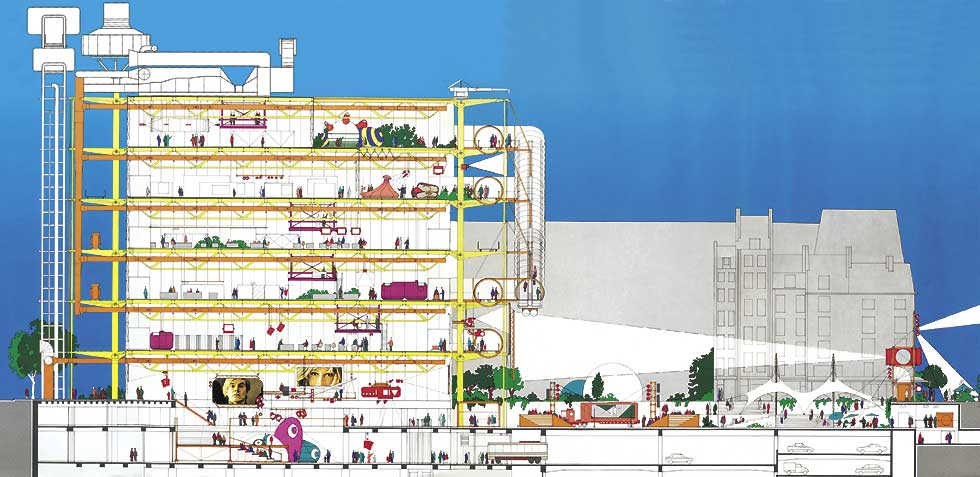
\includegraphics[width=\textwidth]{Illustrations/centre_pompidou.jpg}
    \caption[Centre Pompidou,(1971)]{An initial design drawing sketches imagines a building projection (marked through a white cone) onto the main facade in front of the main plaza. Smaller projections were suggested indoors projecting onto the outer front.}
    \label{centre_pompidou}
\end{figure}

%%%%%%%%%%%%%%%%%%%%%%%%%%%%%


What is missing here is: Venturi, Learning from Las Vegas (1972)
Learning from Las Vegas (1972) created a healthy controversy on its appearance in 1972, calling for architects to be more receptive to the tastes and values of "common" people and less immodest in their erections of "heroic," self-aggrandizing monuments.
Quote: “The Signs, oriented towards the driver’s view, use all kinds of media simultaneously: words, pictures, architecture, sound, light. The whole and its parts are balanced to work from far and near, at day and night.”


%%%%%%%%%%%%%%%%%%%%%%%%%%%%%
\subsubsection{Architectural Lighting}

Before actually continuing with electronic surfaces I briefly discuss the topic of architectural lighting which is important to mention as it existed as a discipline long before the use of electronic surfaces.

%%%%%%%%%%%%%%%%%%%%%%%%%%%%%

\begin{figure} [h!]
    \centering
        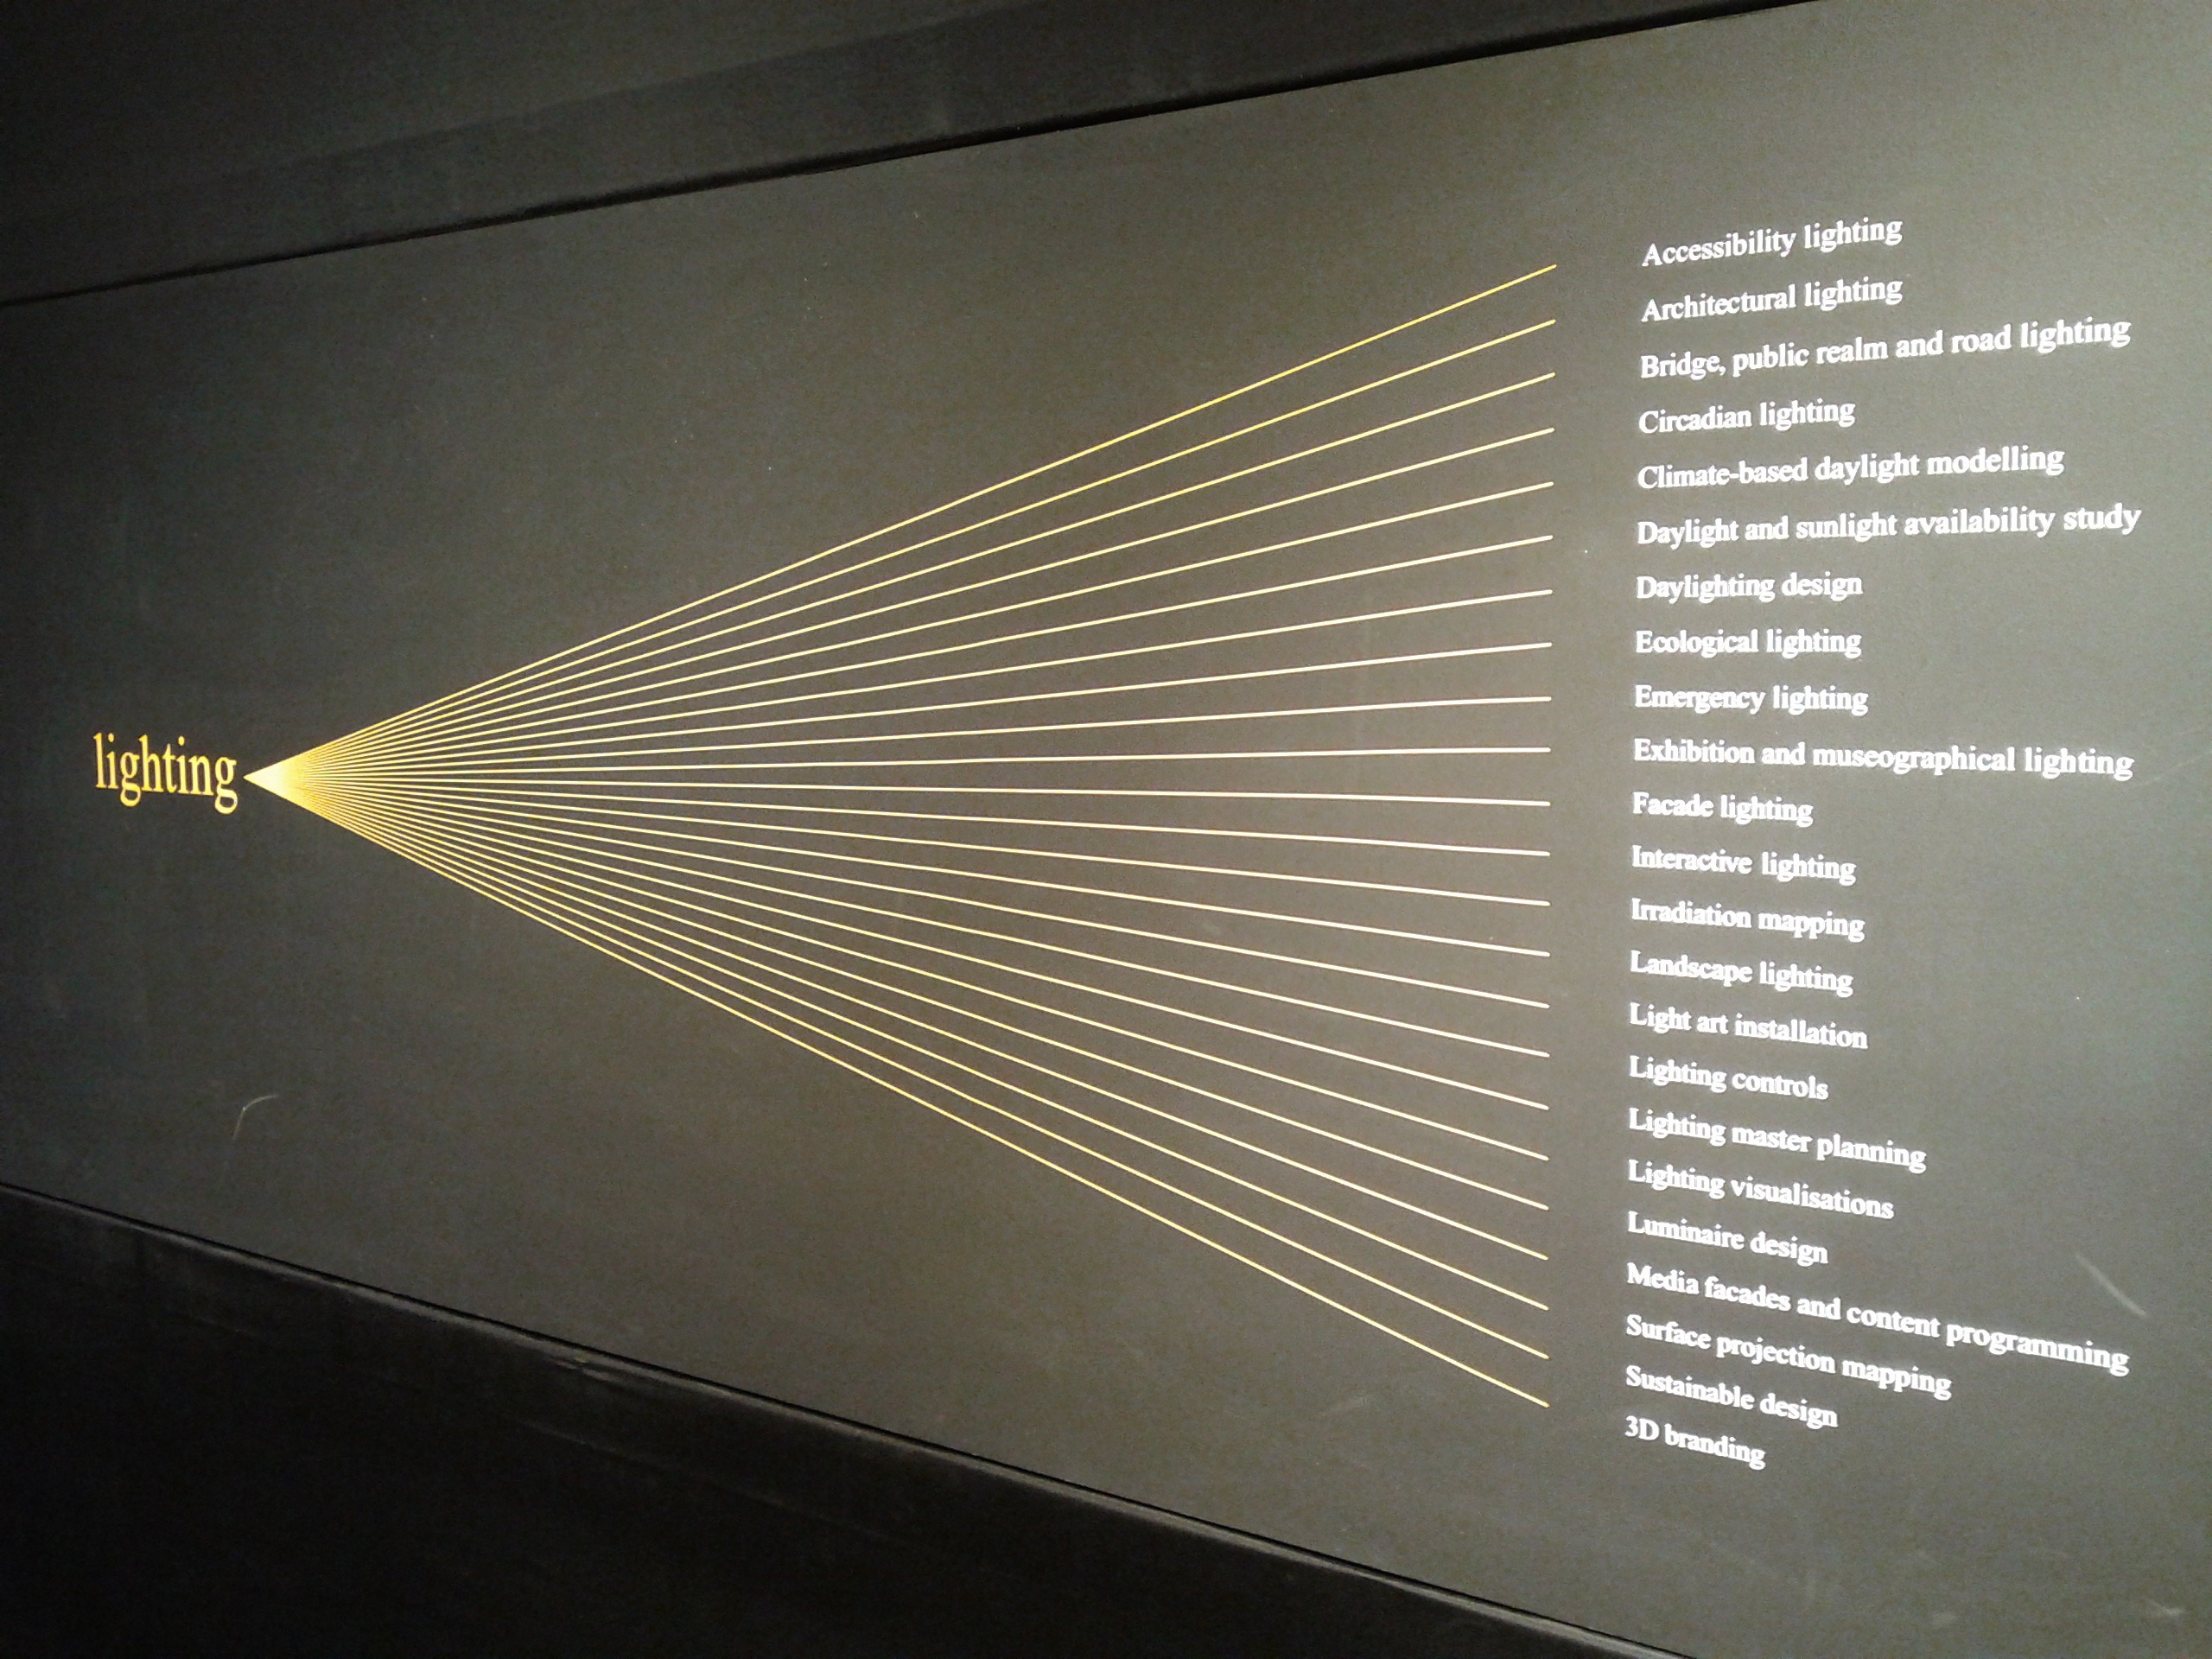
\includegraphics[width=12cm]{Illustrations/Architectural-Lighting-Fields.jpg}
    \caption[Fields of Architectural Lighting]{This diagram has been compiled by Arup for their exhibition on lighting during the international year of light in 2015 \footnote{http://www.light2015.org} }
    \label{InterfacingArchitecture}
\end{figure}

%%%%%%%%%%%%%%%%%%%%%%%%%%%%%

%%%%%%%%%%%%%%%%%%%%%%%%%%%%%

\subsection{Facade as Medium}

When it comes to architecture the notion of a building's front has always had an informational value - although static. A facade was considered to be an interface that connects the bourgeoisie (private space) with the surrounding city (public space) (Neumeyer, 2002). Architectural facades \index{architectural facade} have always been information carriers. (Architecture as a Mass Medium,  Renato De Fusco 1967)
In McLuhan's understanding traditional building materials such as bricks and stones are the medium out of which ornaments and sculptures are formed to communicate the building owner's profession or social status. 
When new media technologies emerged new types of facades emerged \cite{Haeusler2009}. Amongst those light-emitting diodes (LED) appeared as a material to build (dynamic) light facades. 
Building envelopes turned into large programmable pixel matrices displaying animated visual patterns. Information is literally not set in stone any more. 
On the contrary one can argue that new media technologies as a material in architecture has led to an arbitrary and constant exchange of information and as such can lead to a loss of identity of the built environment. Identity of place is an important feature in designing functional public spaces (see \ref{placemaking}). 

At the same time the nature of anytime and anywhere information access changed the relation between the public and private spaces which led to the development of novel forms of interactions between humans and humans, humans and computers and humans and architecture. Whereas Manovich clearly states that HCI is interactive per se (Manovich, 1991, p.71), architecture is not yet. A scale of interactivity has been described by Fritsch and Brynskov (2011) and extended by Caldwell et al. (2014).

%Manovich suggests to have a look at computer science to understand what is media today.
%To understand the logic of new media we need to turn to computer science. It is there that we may expect to find the new terms, categories and operations which characterize media which became programmable. From media studies, we move to something which can be called software studies; from media theory — to software theory.

Meanwhile, digital media technology has been weaved into buildings’ surfaces. 
For instance, visually animated surfaces, such as dynamic light facades, have been equipped with numerous addressable light-emitting diodes (LED). The FIESP building in Sao Paulo, which will be discussed in detail in the case study, is fitted with such a façade. 
Only recently the iconic 1970s building on Avenida Paulista was extended by a large programmable pixel matrix, which displays animated visual patterns. 
From a technical perspective there are other types of large electronic surfaces as well, such as projections onto facades (i.e. building projections), DIY displays, urban screens, media facades or media architectures, which I will discuss in detail in the next section.

%%%%%%%%%%%%%%%%%%%%%%

% - pre-historic cave paintings - Semper
%- Critique about the mere visual sense in today's production of architecture: Media architecture – participation through the senses Katarzyna Urbanowicz
%- In this respect the visual dominance of the visual senses have to be mentioned here. Juhani Pallasmaa (2005, 10) in his book “The Eyes of the Skin”, aims “to create a conceptual short circuit between the dominant sense of vision and the suppressed sense modality of touch.” In a way this aim is summarising the idea of interactive media architecture in my dissertation. 
%- dynamic light facades, that are equipped with numerous light-emitting diodes (LED). They turn into large programmable pixel matrices displaying animated visual patterns \cite{Haeusler2009}. 
%- today we aim to merge the digital technologies with the physical structures to enhance the urban experience  
%- "In a certain sense, the screen became the last wall. No wall out of stone, but of screens showing images. The actual boundary is the screen."  Paul Virilio, 1993 in an  interview with ‘Architecture in the Age of its Virtual Disappearance’

%%%%%%%%%%%%%%%%%%%%%%


\subsection{Large Electronic Surfaces}

Large programmable electronic displays such as building projections, urban screens, media facades and media architecture are increasingly dominating the mediascape of our cities for various purposes such as information communication, navigation, advertising and occasionally for media art. 
Today it seems that due to their omnipresence large programmable displays need to go beyond commercial purposes to stand out and create value.
At the same time electronic surfaces became a material to support architectural concepts and to implement structures. Price decline allows non-commercial initiatives to embed displays for their purposes. 
In this respect the EU funded Connecting Cities Network (CCN) established an ecology of test beds that connects various electronic surfaces and their stakeholders around the globe with enthusiastic media technologists and artists. 
Consequently, this novel synergy offers a unique opportunity for contemporary media art to explore novel socio-technological practices in urban spaces. 
It is a promising prospect to regain urban public space as the participatory domain within our cities. 
In this, novel digital technologies may support participation and media art is spearheading the exploration into interactive systems that may evoke new practices for a participatory city. 
In the following I will describe the evolution of electronic surfaces in research and practice.
I focus in particular on large programmable displays in public spaces such as public displays, urban screens, building projections, media facades or media architectures. I will consider their constituting elements potential for mediating social interactions.

%%%%%%%%%%%%%%%%%%%%%%%%%%%%%

\begin{figure} [h!]
    \centering
        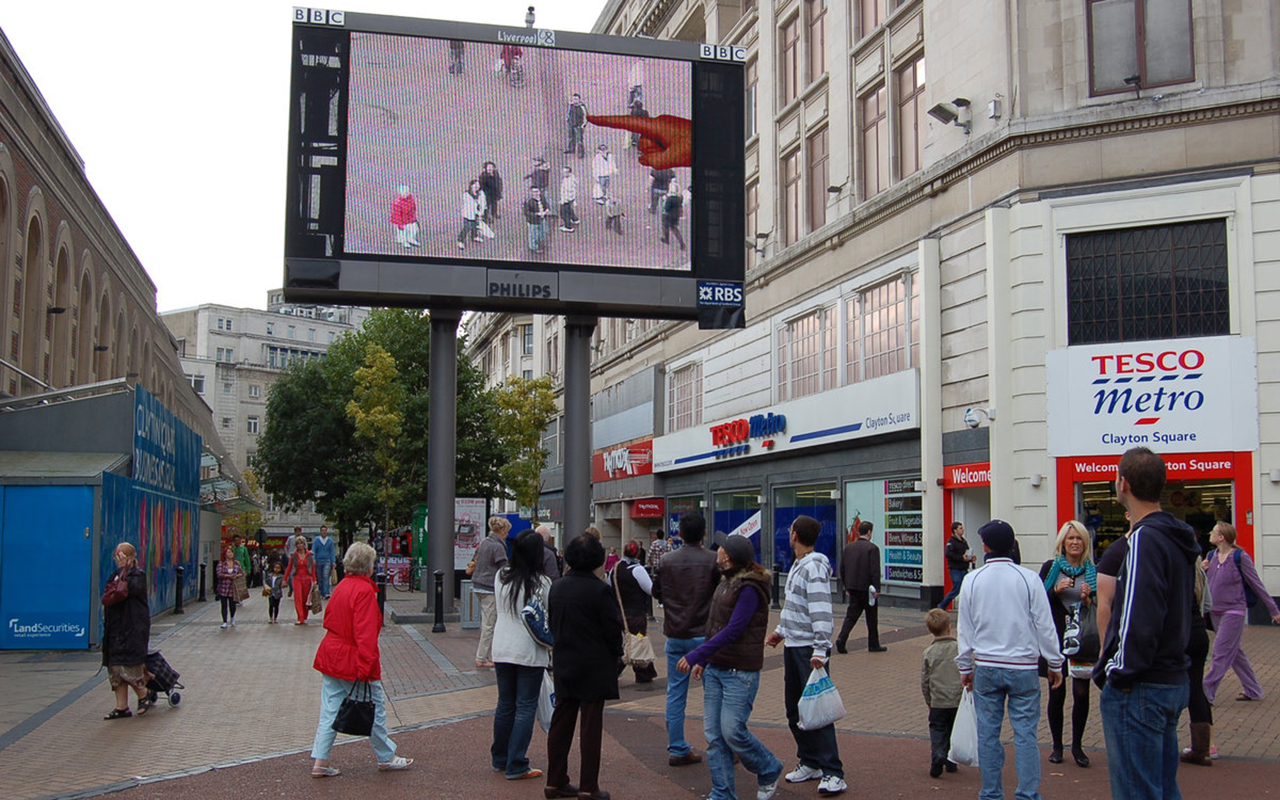
\includegraphics[width=4.5cm]{Illustrations/3.jpg}
        	%\caption[a]{Urban Screen}
      	%\label{UrbanScreen}
        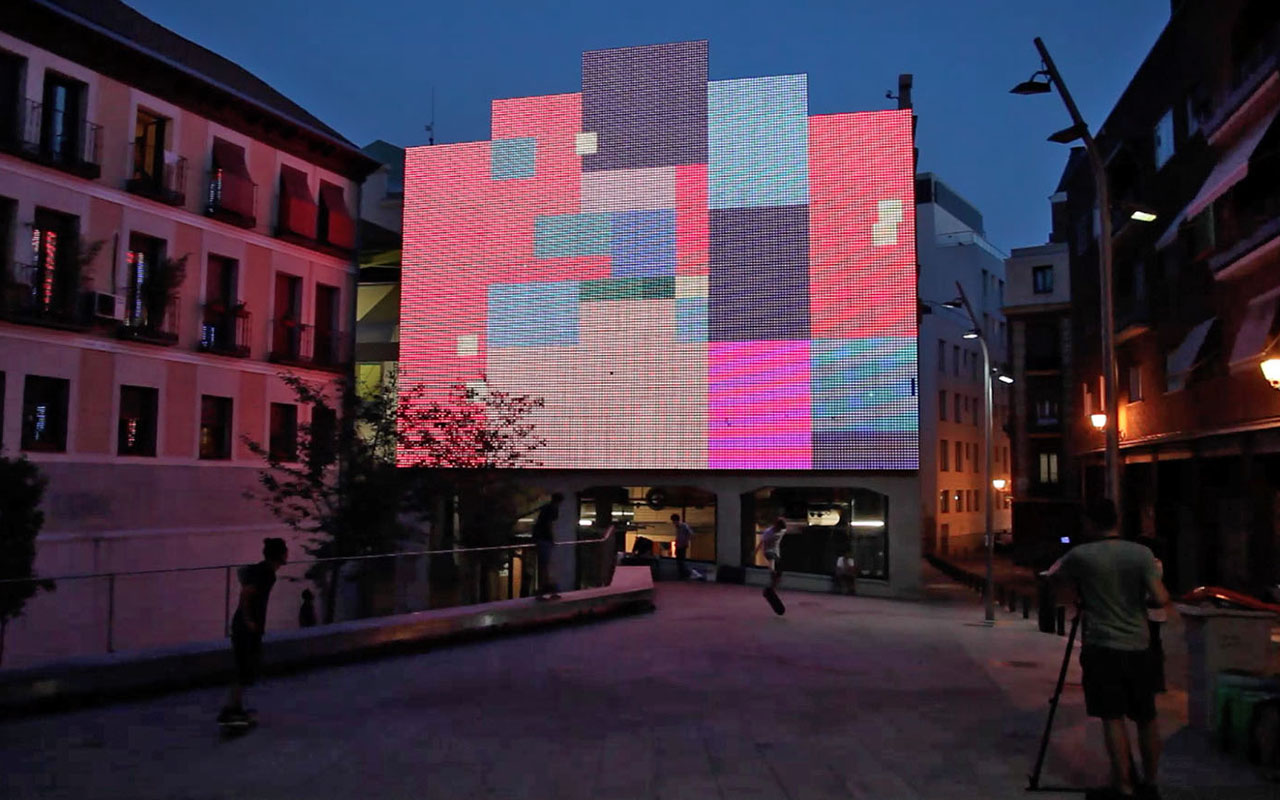
\includegraphics[width=4.5cm]{Illustrations/2.jpeg}
       		%\caption[b]{Media Facade}
       	%\label{MediaFacade}
        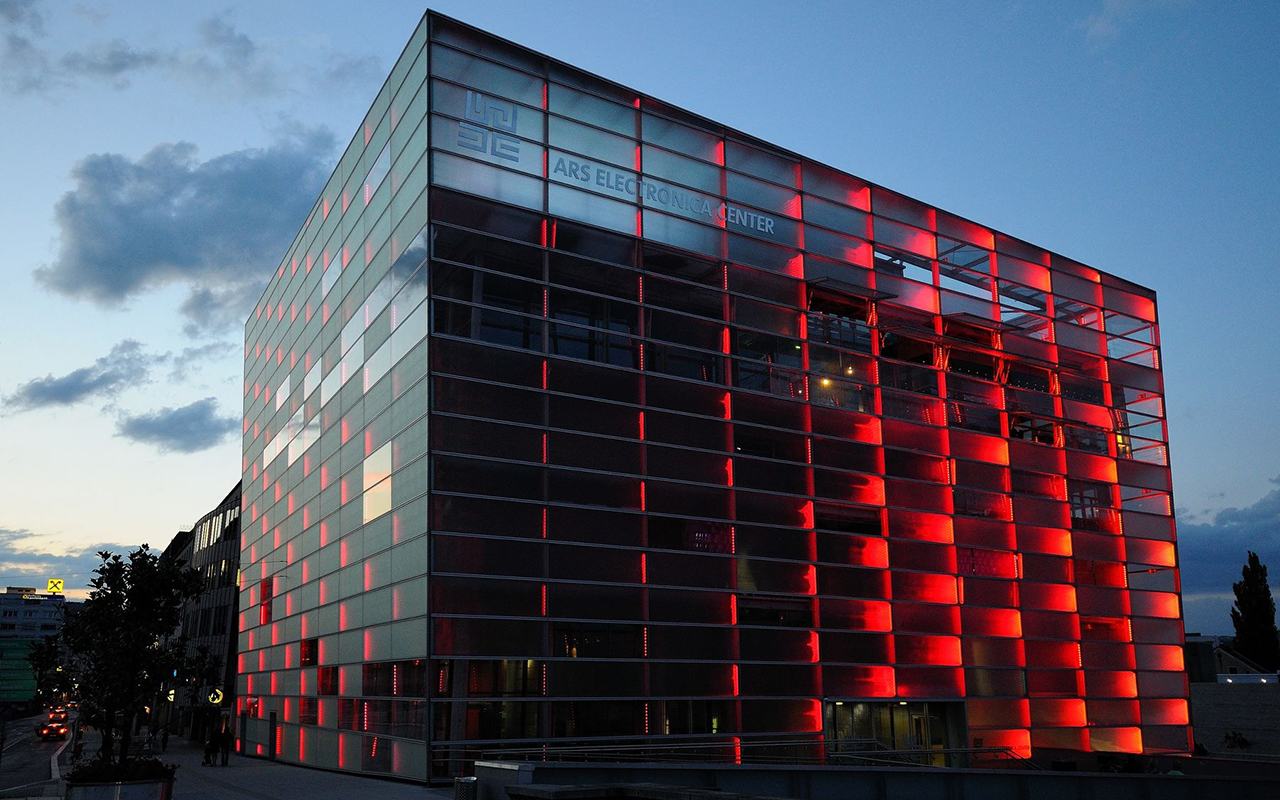
\includegraphics[width=4.5cm]{Illustrations/1.jpg}
       		%\caption[c]{Media}
     	%\label{MediaArchitecture}
    \caption[Types of electronic surfaces]{Types of large electronic surfaces in public space: (left) a free-standing rectangular urban screen, (middle) a individually shaped media facade, (right) a low resolution media architecture}
    \label{InterfacingArchitecture}
\end{figure}

%%%%%%%%%%%%%%%%%%%%%%%%%%%%%


% Please add the following required packages to your document preamble:
% \usepackage{graphicx}
\begin{table}[H]
\centering
\resizebox{\textwidth}{!}{
%\setlength{\extrarowheight}{10pt}
\setlength{\extrarowheight}{10pt}

\begin{tabular}{l|l|l|l} 
\multicolumn{1}{c|}{\textbf{Type of surface}} & \multicolumn{1}{c|}{\textbf{Surface properties}} & \multicolumn{1}{c|}{\textbf{CCN infrastructure}} & \multicolumn{1}{c}{\textbf{CCN project}} \\ \hline

\textit{Human Displays}& \begin{tabular}[c]{@{}l@{}}- embodied \\ - mobile \\ - indoors or outdoors\end{tabular} & - public space  & - 'Master/Slave Invigilator System', Jeremy Bailey (2013)  \\ \hline

\textit{Urban Screens}  & \begin{tabular}[c]{@{}l@{}}- situated \\ - permanent or temporary \\ - stand-alone or mounted\end{tabular} & \begin{tabular}[c]{@{}l@{}}- BBC Big Screen, Liverpool\\- Beşiktaş Square, Istanbul\end{tabular} & \begin{tabular}[c]{@{}l@{}}- 'Hand from Above', Chris O’Shea (2010)\\- 'Connecting Monsters', HDOTO (2013)\end{tabular}  \\ \hline

\textit{Media Facades}  &- embedded or retrofitted & \begin{tabular}[c]{@{}l@{}}- Medialab Prado, Madrid \\ - Galeria de Arte Digital do SESI-SP, Sao Paulo\end{tabular} & \begin{tabular}[c]{@{}l@{}}- ‘Sonic Skate Plaza’, Pablo Serret de Ena (2013) \\ - ‘G-Frame’, The Constitute (2014)\end{tabular}     \\ \hline

\textit{Media Architecture}  & - multi-dimensional & - Ars Electronica Centre, Linz  & \begin{tabular}[c]{@{}l@{}}- ‘Smart Citizen Sentiment Dashboard’, Behrens/Valkanova (2014)\\ - ‘(We are) Light Catchers’ Michael Ang (2015)\end{tabular}
\end{tabular}%
}
\caption[Types of electronic surfaces in urban space]{Types of electronic surfaces in urban space demonstrated through selected projects from the CC Network.}
\label{tab:typesofsurfaces}
\end{table}

%%%%%%%%%%%%%%%%%%%%%%%%%%%%%

% Please add the following required packages to your document preamble:
% \usepackage{graphicx}
%\begin{table}[]
%\centering
%\resizebox{\textwidth}{!}{
%\setlength{\extrarowheight}{10pt}

%\begin{tabular}{l|l|l|l|l}
%surface & \textbf{Human Display} & \textbf{Urban Screen} & \textbf{Media Facade} & \textbf{Media Architecture} \\ \hline
%properties & \begin{tabular}[c]{@{}l@{}}- embodied\\ - mobile\\ - indoors or outdoors\end{tabular} & \begin{tabular}[c]{@{}l@{}}- situated\\ - permanent or temporary\\ - stand-alone or mounted\end{tabular} & - embedded or retrofitted & - multi-dimensional \\ \hline

%infrastructure & \begin{tabular}[c]{@{}l@{}} - public space \end{tabular} & \begin{tabular}[c]{@{}l@{}}- BBC Big Screen, Liverpool\\ - Beşiktaş %Square, Istanbul\end{tabular} & - Galeria de Arte Digital do SESI-SP, Sao Paulo & - Ars Electronica Centre, Linz  \\ - Media Lab Prado \\ \hline

%project & \begin{tabular}[c]{@{}l@{}} 'Master/Slave Invigilator System', Jeremy Bailey (2013) \end{tabular} & \begin{tabular}[c]{@{}l@{}}- 'Hand from Above', Chris O’Shea (2010)\\ - 'Connecting Monsters', HDOTO (2013)\end{tabular} & - ‘Sonic Skate Plaza’, Pablo Serret de Ena (2013)\\ - ‘G-Frame’, The Constitute (2014)- ‘Smart Citizen Sentiment Dashboard’, Behrens/Valkanova (2014)\\ - ‘(We are) Light Catchers’ Michael Ang (2015) \\ \hline

%\end{tabular}%
%}
%\caption{My caption}
%\label{my-label}
%\end{table}

%%%%%%%%%%%%%%%%%%%%%%%%%%%%%

%\begin{figure}[!h] 
%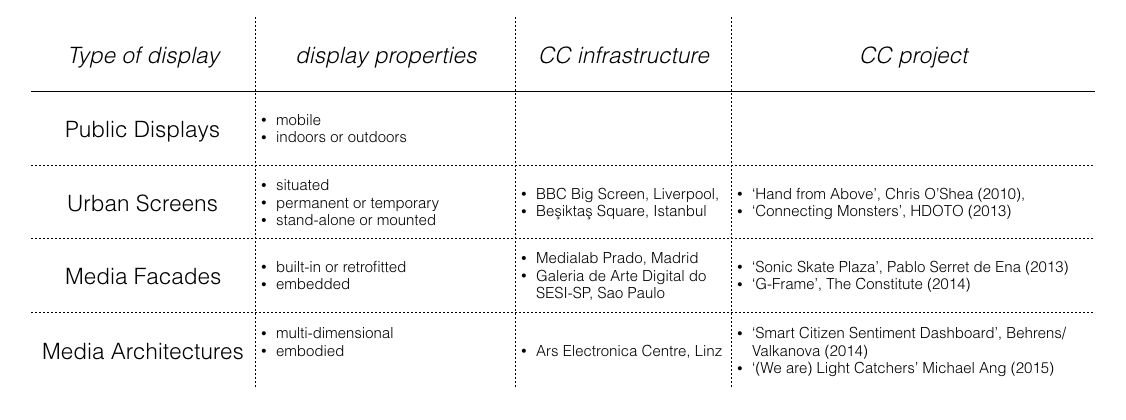
\includegraphics[width=\textwidth]{Illustrations/Types-of-displays.png}
%\caption{Types of displays}
%\label{fig:lion}
%\end{figure}

%%%%%%%%%%%%%%%%%%%%%%%%%%%%%%

\subsubsection{DIY Displays and Temporary Media Architectural Installations}

A specific application of media architecture that allows for a more experimental approach towards the exploration of new electronic surfaces are temporary media architectural installations. Due to their temporary implementation they are excluded from sometimes cumbersome processes.

\begin{itemize}
\item "Lichtwolke" - Raumwelten \index{Lichtwolke - Raumwelten (2016)} is a temporary blow-up structure that even allows for people to inhabit the structure 
\item  \textit{SKUM} \index{SKUM (2016)} by BIG architects = "inflatable balloon pavilion by bjarke ingels group / BIG. named ‘SKUM’ – the danish word for ‘foam’ – the playful and bubble form was first erected at the roskilde festival and uses the same material as bouncy castles" (taken from website).
\end{itemize}

The projects I have developed within the scope of this dissertation can be considered as temporary media architecture. They allow to be of structural and architectural nature but at the same time - through their temporarity - they give a maximum of experimental and prototypical flexibility. 


With a rapid price decline and the development of open-source platforms that provide easy to learn software tools such as Processing and Arduino computational designing became more accessible for non-experts 

With the advent of the www knowledge spread and made available more easily. Online platforms and communities provide, exchange and create new knowledge accessible for laypeople. Today we can easily find answers on how-to-fix problems, get instructions on how to do-it-yourself (DIY) or join a community and do-it-with-others (DIWO) . DIY and the maker movement not only became an alternative to consumerism but also for researchers and designers to enter new domains or to integrate digital technologies into their design work.  
One of those domains include urban computing technologies and media such as public displays. 
Access to DIY cultures and knowledge in the context of networked public displays has been used to explore community engagement by a collaboration between researchers from UCL The Bartlett and the Mixed Reality Lab at the University of Nottingham in the EPSRC funded Screens-in-the-Wild \index{Screens in the Wild (2011)} project. 
%(Considering communities, diversity and the production of locality in the Design of Networked Urban Screens by Wallis Motta https://www.irit.fr/recherches/ICS/events/conferences/interact2013/papers/8117312.pdf)

DIY Media Architectures have been explored by Caldwell et al. (2014) (DIY media architecture: Open and participatory approaches to community engagement. Caldwell, Glenda Amayo ; Foth, Marcus (2014)) 
They categorised DIY maker cultures with respect to media architectures into three categories, namely, \textit{technical DIY} which refers to the maker cultures themselves, \textit{spatial DIY}, which describe "urban interventions for the purpose of appropriating public spaces to assist in civic engagement, the communication of often political messages, or to simply improve the quality and experience of a place." (Caldwell et al.) and can be summarised with the term placemaking. The third category is called \textit{social DIY}, which they summarize as urban citizenship.

Recent projects that include DIY displays include. I have categorised them following the framework Caldwell et al. suggested:

\begin{itemize}
\item Heart of the City http://www.connectingcities.net/project/heart-city
\item (WE ARE) LIGHT CATCHERS http://www.connectingcities.net/project/we-are-light-catchers
\end{itemize}

%%%%%%%%%%%%%%%%%%%%%%%%%%%%%

Different kind of display - so called drone displays - has been explored by Ars Electronica in the project \textit{Spaxels} \index{Spaxels} \index{Ars Electronica} \footnote{\url{http://www.spaxels.at/} accessed 07.12.2016}

%%%%%%%%%%%%%%%%%%%%%%%%%%

\begin{figure}[htp]
\centering
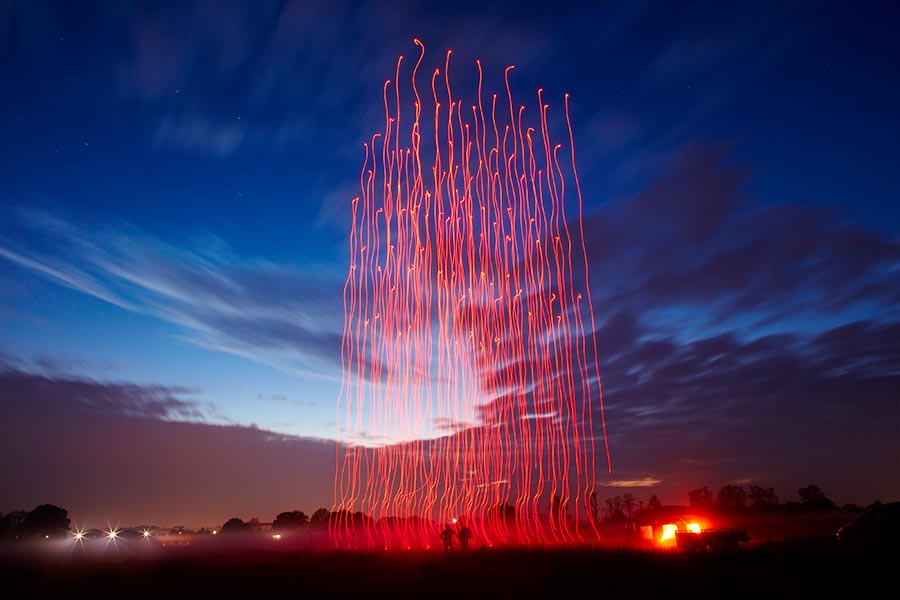
\includegraphics[width=\textwidth]{Illustrations/spaxels.jpg}
\caption{A series of drones equipped with LED pixels form a dynamic display.}
\label{spaxels}
\end{figure}

%%%%%%%%%%%%%%%%%%%%%%%%%%

The VEIV display that is part of the case study in this dissertation can be described as an DIY display. The purpose was to test an idea in an affordable time and cost frame, without specific knowledge. Based on the observations of the implementation I was able to develop a research proposal for this PhD.

DIY practices may encourage digital literacy amongst citizens in the smart city at the same time they allow interdisciplinary research. 

%%%%%%%%%%%%%%%%%%%%%%%%%%%%%%


\subsubsection{Building Projections}

For the initial proposal of the Centre Pompidou \index{Centre Pompidou (1971)} in 1971 Rogers and Piano envisioned a large projection onto the main facade of the cultural centre announcing the programme of what is going on inside (Fig.\ref{centre_pompidou}).  

Building projections map dynamic content onto existing architectural facades by means of an optical device that projects (animated) images onto a surface. Projection mappings are mostly temporary and designed for special occasions. They aim to augment architectural facades with additional dynamic visual content - mostly with a strong narrative.  

Large building projections became popular among light festivals where historic iconic building facades such as churches are overlayed with colourful patterns. Currently the biggest of these nocturnal events is the VIVID Light Festival in Sydney, Australia, where each year millions of visitors are fascinated by the various light shows and building projections produced with the latest projection technology. Light festivals in the meanwhile belong to the repertoire of global city marketing hence many major city is organising an annual festival. The first festival of this kind emerged in the French city of Lyon \footnote{Since 1852 the citizens of the French city Lyon are coming together to celebrate the unity of their city with a light festival called La Fete des Lumieres. Back then candle lights were positioned in each window. Since 1999 a professional light festival attracts many tourists in Dezember to visit Lyon. See also: \url{http://www.fetedeslumieres.lyon.fr/en/page/history} accessed 04.11.2016}.    

A building projection project worth mentioning here is the \textit{555 KUBIK} \index{555 KUBIK (2009)} project initiated by the German based \textit{Urbanscreen} agency for the facade of the Hamburger Kunsthalle, Galerie der Gegenwart in 2009 \footnote{\url{http://www.urbanscreen.com/555-kubik/} accessed 10.11.2016}. The content of full facade projection successfully plays with the existing architectural surface.  

%%%%%%%%%%%%%%%%%%%%%%%%%%

\begin{singlespace}
	\leftskip2.3em
		\rightskip\leftskip
\textit{\small The Basic idea of narration was to dissolve and break through the strict architecture of O. M. Ungers “Galerie der Gegenwart”.
Resultant permeability of the solid facade uncovers different interpretations of conception, geometry and aesthetics expressed through graphics and movement. A situation of reflexivity evolves – describing the constitution and spacious perception of this location by means of the building itself.} 

\small Project description by Urbanscreens
\end{singlespace}

%%%%%%%%%%%%%%%%%%%%%%%%%%

What is interesting here is that the designers of the projection content were playing with the rigid design grid O.M. Ungers is famous for. The rigid facade was augmented through the projection. In contrast to many other building projections here the augmented content and the original facade seemed to merge and graphical additions seemed to extend the facade.

%%%%%%%%%%%%%%%%%%%%%%%%%%

\begin{figure}[htp]
\centering
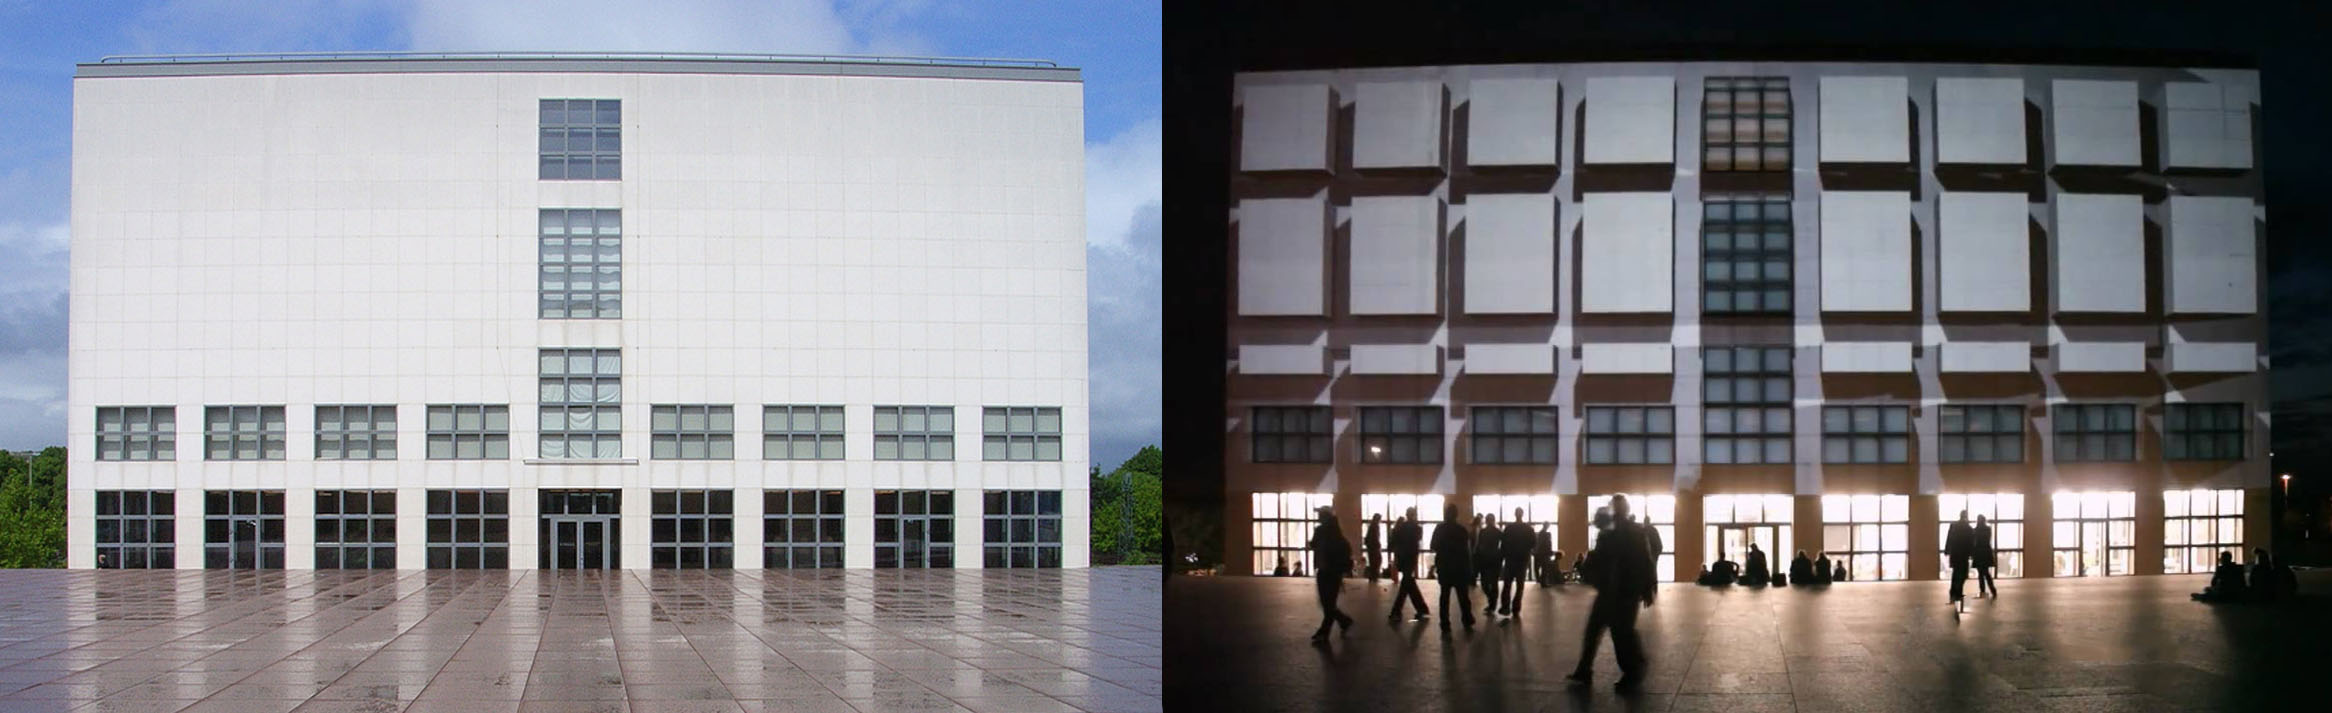
\includegraphics[width=\textwidth]{Illustrations/Ungers_day_night.jpg}
\caption{Augmentation of an architectural facade through a projection. The dynamic content allows for a speculative extension of the given surface.}
\label{fig:ungers}
\end{figure}

%%%%%%%%%%%%%%%%%%%%%%%%%%

Besides the common facade mappings there are a few so called rear-projections, that project content onto translucent film from the back. An installation that has been developed permanently and has been part of the initial architectural design process is the Media Wall.
The Media Wall in the IAC Building in New York designed by Frank Gehry and completed in 2007 is built into the reception area. 
Its dimensions are 3.4 meters high and 37 meters long. 
The projectors are based on Laser Phosphor Display (LPD) technology \footnote{ \url{http://www.prysm.com/laser-phosphor-display accessed 10.11.2016}}
Thin laminated film sandwiched between glass panels enable high resolution that compared to LED displays allows for very close use of participants.
This rear projection project is different to others and mentioned here as it is not a temporary installation with a removable support structure. The project had to be integrated into the building structure itself early on. The section Fig .. shows the backstage of the display wall with scaffolding, mirrors and projectors.

Content wise projection mappings do not always serve merely the purpose to entertain an audience with colourful and flashy animation as widely demonstrated in light festivals.   
Political activism was first explored through projections by pioneering artist Krzysztof Wodiczko, who projected a swastika on the South Africa  embassy  in Trafalgar Square London in 1985 to confront former PM Thatcher over financially supporting the  apartheid regime. Although the projection lasted only two hours the impact and media coverage has been overwhelming.     
During the 2011 Occupy Wall Street protests building projections have been used by the New York activist group The Illuminator \footnote{\url{http://theilluminator.org/about/}} to map the movements 99percent logo onto the iconic Verizon building. 

%%%%%%%%%%%%%%%%%%%%%%%%%%

\begin{singlespace}
	\leftskip2.3em
		\rightskip\leftskip
\textit{\small "99\% / MIC CHECK! / LOOK AROUND / YOU ARE A PART / OF A GLOBAL UPRISING / WE ARE A CRY / FROM THE HEART / OF THE WORLD / WE ARE UNSTOPPABLE / ANOTHER WORLD IS POSSIBLE / HAPPY BIRTHDAY / \#OCCUPY MOVEMENT / OCCUPY WALL STREET / {[list of cities, states and countries]} / OCCUPY EARTH / WE ARE WINNING / IT IS THE BEGINNING OF THE BEGINNING / DO NOT BE AFRAID / LOVE."} 

\small As the demonstration took the Brooklyn Bridge The Illuminator supported the chanting protest march with these messages.
\end{singlespace}
\
%%%%%%%%%%%%%%%%%%%%%%%%%%

The group developed a projector van, which allowed them to project the 99percent logo onto any facade in New York with ease.

Building projections can also be interactive as shown by the SMSlingshot project. Here participants were invited to shoot text messages onto a facade with the use of a slingshot.  
On another matter projections have been used for prototyping social data visualisations in favour of public engagement. Valkanova et al. (...) developed an application asking participants to reveal their energy consumption data publicly which is then projected onto a public wall. The aim is to enable rich discussions about energy consumption and behaviours.  

Projections on different surfaces: 

In summary, the small size of projectors, their high mobility and ability to be set up quickly with projecting from various angles they are highly suitable for rapid urban prototyping, bottom-up initiatives and political activism.  Consequently they have a very strong temporal aspect.
Their high resolution allow for close distant interactions.
Only occasionally the specific form of rear projections is used in permanent architectural set ups.

%%%%%%%%%%%%%%%%%%%%%%%%%%%%%

\subsubsection{Urban screens}

Urban screens are considered to be a technological advancement of the traditional billboard, serving to broadcast commercial content \cite{Huhtamo2009}. 
In the 1970s James P. Mitchell's invention of a LED (light emitting diode) matrix marked the end of the analog CRT displays (cathode-ray tube technology). This novel display technology paved the way towards today's high-resolution outdoor public displays, called urban screens.
Whilst public displays include TV sized screens in indoor places such as museums urban screens are different in scale and considered to be outdoors. 
Large programmable electronic surfaces such as urban screens can be stand-alone or façade-mounted whilst being used either temporary or permanent (Tscherteu and Tomitsch, 2011). 
%Tscherteu and Tomitsch describe urban screens as mid- to large-scale screens that can either be freestanding or attached to a building façade. (Tscherteu, G.  Tomitsch, M. (2011). Designing Urban Media Environments as Cultural Spaces. Presented at the CHI’11 Workshop on Large Urban Displays in Public Life, May 2011, Vancouver, Canada.)
In 2005 a conference was hosted in Amsterdam with the name Urban Screens. For the first time advertisers, content providers, engineers, stakeholders, researchers, architects, city planners and artists came together to discuss the future of large public displays. 
The questions considered since then were manigfold:

%%%%%%%%%%%%%%%%%%%%%%%%%%%

\begin{singlespace}
	\leftskip2.3em
		\rightskip\leftskip
\textit{\small "What is the relation between technology, culture, economics and politics? How do technical decisions, such as determining standards and ‘affordances’, or erecting stand-alone installations or forming unified networks, affect cultural experiences and the distribution of power? How should we conceptualise public participation in relation to urban screens? Are the public citizens, consumers, producers, or something else? And when considering the location of a large screen, what are the appropriate forms of urban planning, design and governance? When a screen is erected in public space, who should have access to it and who has control over it? What kinds of partnerships enable innovative screen programs, and contribute to rich public cultures? How might this be evaluated? In what conditions can public screens contribute not only to new forms of public interaction but to the deeper democratic ambi- tions of public culture? Where is the contemporary public sphere located and what are its boundaries and lines of force?"} 

\small Taken from the introduction of the Urban Screens Reader by Mcquire, S., Martin, M. and Niederer, S. 2009.
\end{singlespace}

%%%%%%%%%%%%%%%%%%%%%%%%%%%

One can mention the stand-alone and permanent \textit{BBC Big Screens} \index{BBC Big Screens} distributed across the UK. In Liverpool the Big Screen hosted a CCN project in 2010 named \textit{Hand from Above} \index{Hand from Above (2010)} by Chris O’Shea.
A similar infrastructure exists at the Beşiktaş Square in Istanbul where CCN deployed \textit{Connecting Monsters} \index{Connecting Monsters (2013)} by HDOTO in 2013. 

%%%%%%%%%%%%%%%%%%%%%%%%%%%%%

\subsubsection{Media facades}

Haeusler, M. Hank, Tomitsch, Martin,  Tscherteu, Gernot. (2013). New Media Facades: A Global
Survey. Ludwigsburg, Germany: avedition.

Another type of large electronic displays constitutes media facades. Here digital media technology is already built-into the building’s surface or retrofitted to an already existing building. An example where the installation of a media facade was already part of the initial design process of the building is the Media Lab Prado in Madrid, Spain or the Ars Electronica Center in Linz, Austria. Whereas the iconic FIESP building in Sao Paulo, Brazil built in the 1970s only recently was retrofitted with a media facade.

Seen from building engineering, according to Tomitsch, media facades "in contrast to Urban Screens feature a closer integration of the screen and the building layers, if not a complete integration into a new hybrid structure." (Tomitsch)

Eight challenges have been identified by Dalsgaard and Halskov (2010). 
%Dalsgaard, P., & Halskov, K. (2010). Designing Urban Media Façades: Cases and Challenges. In Proceedings of the 28th international conference on Human factors in computing systems (pp. 2277–2286). ACM.
These challenges clearly acknowledge the importance of the particular physical space a media facade is planned to be implemented (i.e. Spatial Layout). Further the impact of media facades on social interactions (i.e. Movement) is mentioned, as well as the function of the media facade itself (i.e Attractor).
%%%%%%%%%%%%%%%%%%%%%%%%%%

\begin{figure}[htp]
\centering
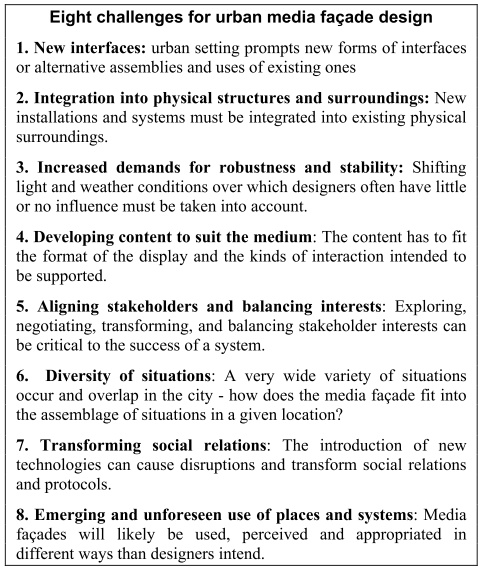
\includegraphics[width=8cm]{Illustrations/8challenges.png}
\caption[Eight challenges for urban media facade design]{Eight challenges for urban media facade design taken from }
\label{8challenges}
\end{figure}

%%%%%%%%%%%%%%%%%%%%%%%%%%

Kunsthaus Graz \index{Kunsthaus Graz - BIX (2003)}finished in 2003 is an architectural landmark designed by Archigram architect Peter Cook and Colin Fournier. 
The BIX {(acronym for Big piXels)} media facade has been designed by the Edler brothers from the Berlin based practice realities:united 
%\footnote{\url{http://www.realities-united.de/#PROJECT,69,1} accessed 11.11.2016}.
In away the BIX media facade is a retrofitted facade as well as the lighting designers have been called in only when the Kunsthaus has already been under construction. Hence in my definition it is not a media architecture. I will explain this in the next section.

The conceptual idea for the BIX media facade has been further explored in the project SPOTS \index{SPOTS (2005)}

A recent project that illustrates the idea of display technology as a material for architectural design is the \textit{LED Frieze} facade (2016) \index{LED Frieze (2016)} for the new building of the Kunstmuseum Basel designed by Christ and Gantenbein. The solid bright brick front with few openings is at the top interrupted with a luminous band of three meters hight that encricles the entire museum at a height of 12 meters. The relief like pattern of the bricks creates tiny voids that are equipped with 
The low resolution and monochromatic media facade is able to show text and patterns. From an architectural point of view this is a very successful project.
\smalltodo[size=\footnotesize]{This argument needs to be picked up in the discussion about the cocoon and its appearance ... low res and monochromatic, but very strong in its architectural expression.}
%%%%%%%%%%%%%%%%%%%%%%%%%%

\begin{figure}[htp]
\centering
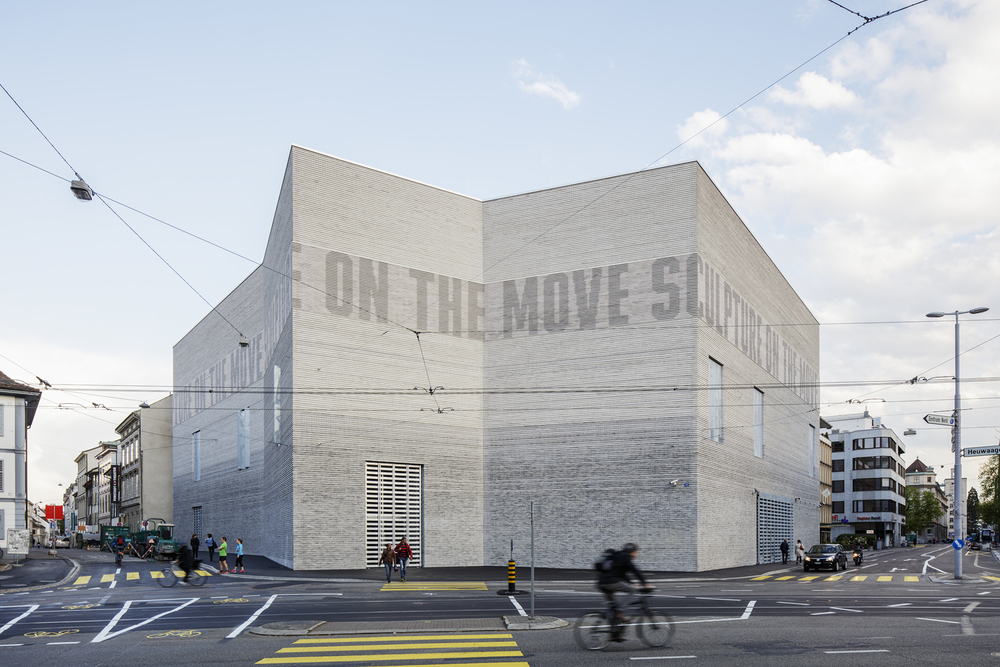
\includegraphics[width=\textwidth]{Illustrations/LEDfrieze.jpg}
\caption[LED Frieze by Christ and Gantenbein (2016)]{xxx}
\label{LEDfrieze}
\end{figure}

%%%%%%%%%%%%%%%%%%%%%%%%%%


\subsubsection{Media architecture}

Although literature in media architectural research mainly considers media architecture as an umbrella for the aforementioned surface types (i.e. DIY screens, urban screens, building projections and media facades), I argue that digital technology and media utilised for architectural design constitutes a category on its own. In the following I will developed a definition for what I consider the notion of media architecture.

In recent years different technical, spatial and social definitions gathered around the emergent term media architecture depending on which discipline is looking at it. Practitioners and researchers from architecture, lighting design, interaction design or HCI covered a wide range of social, spatial and technical aspects. 


The technical aspects with the respect to light have been summarized by Gielen: "Media architectures are technical systems consisting of a matrix of components that are able to individually change its appearance in terms of luminance and/or colour to depict digital content." 
%Johann Gielen (Lighting  Urban Designer, 2013)
The aspect of spatiality in media architectures and how it differs from the aforementioned surface types (i.e. DIY screens, urban screens, building projections and media facades) have been identified by Tomitsch: "Media installations work with the depth of space, in which case it is no longer possible to speak of a screen or a façade." 
%(Tomitsch) 

Brynskov et al. [6: p. 1-2], "Media architecture is an overarching concept that covers the design of physical spaces at architectural scale incorporating materials with dynamic properties that allow for dynamic, reactive or interactive behavior. These materials are often digital, but not always, and they allow architects and (interaction) designers to create spatial contexts for situations using a variety of modalities."
%(Brynskov, M., Dalsgaard, P.,  Halskov, K. (2013). Understanding Media Architecture (Better): One Space, Three Cases. Presented at the CHI’13 Workshop on Interactive City Lighting, Paris, France.)


I consider all these definitions as valuable under the umbrella of media architecture, however they are only describe partially the notion of media architecture. All these definitions together form the notion of media architecture. 

Consequently, media architectures manifest the idea of incorporating digital technologies and media systems already into the initial process of architectural designs by architects, designers and media artists. Here I would like to emphasise the initial intention to integrate digital technologies and media systems as materials of the architect to implement her vision. In other words, media architectures involve multi-dimensional media systems from the very beginning, and electronic surfaces become part of the architectural repertoire. The emblematic building of the Ars Electronica Centre incorporates this approach towards a museum that offers artists the platform to explore the technology mediated future not only within the building but as well on the outer media façade. 

We follow this definition in practice and hence it is part of our methodology in this research.


One can categorise Media Architecture into the following groups as defined by the Media Architecture Institute:
"The Media Architecture Awards are given to outstanding projects at the intersection of architecture, media and interaction design. Three projects are nominated in each of the five categories:

%%%%%%%%%%%%%%%%%%%%%%%%%%%%%

\begin{itemize}
\item \textbf{Animated Architecture:} Projects demonstrating creative media facades solutions
\item \textbf{Money Architecture:} Projects illuminating buildings that are closely related to business, banks, shopping centres, and entertainment.
\item \textbf{Participatory Architecture and Urban Interaction:} Interactive media projects that enable local city development from a bottom up perspective.
\item \textbf{Spatial Media Art and Future Trends and Prototypes:} Projects produced in an artistic context at the intersection of architecture and media art, mostly non-permanent movable installations with an innovative form of spatial interaction and/or perception of space.
\item \textbf{Future Trends and Prototypes:} Special solutions like three-dimensional displays, kinetic facades, OLEDs or even robotic elements that could shed light on what future media architectures might look like.
\end{itemize}



\begin{figure}[htp]
\centering
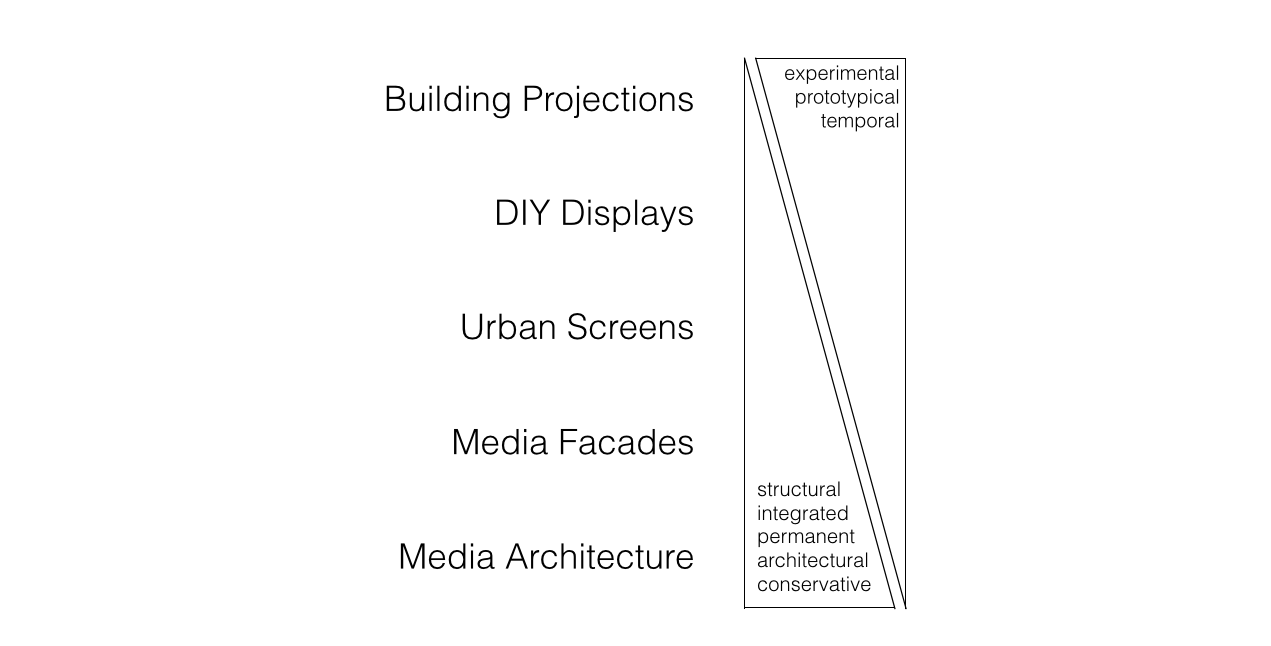
\includegraphics[width=\textwidth]{Illustrations/Typo_diagram.png}
\caption{Interactivity is missing!!! The diagram shows the properties and relations between }
\label{Typo_diagram}
\end{figure}

%%%%%%%%%%%%%%%%%%%%%%%%%%

\subsubsection{Architectural/Urban Mediascapes  / Networked Urban Mediascapes}

Definition:
Marcus Foth, Florian Fischer, Christine Satchell:From Movie Screens to Moving Screens: Mapping Qualities of New Urban Interactions, Media City 4

Projects:
- illuminated river london
- China ... ?

%%%%%%%%%%%%%%%%%%%%%%%%%%

\subsection {Media Architecture and the Role of Context}

McQuire \cite{McQuire2006} argues that TV screens have been transformed from small-scale interior devices to large architectural surfaces that no longer broadcast to private inside spaces but to public outside spaces. Architectural surfaces turned into public media interfaces, transmitting mostly content curated by corporate organisations, rather than interactions generated by the public in situ. 

Some see digital media facades as simple ornaments that create an ambient atmosphere \cite{Caspary2009}. 
Others consider the potential of digital media facades for communicating content, for instance, advertising (e.g. Times Square, New York or Piccadilly Circus, London), news content (e.g. the network of Big Screens in the UK, which was initially run by the BBC),\footnote{xxxBBCBigscreen} media art (e.g. Lozano Hemmer’s work),\footnote{xxx} social visualization (e.g. BlinkenLights)\footnote{xxx} or for community purposes on a neighbourhood level (e.g. Screens in the Wild).\footnote{xxx}

Extensive research has been carried out to explore the challenges of deploying large electronic surfaces in public space.
Initially, the technical challenges of deploying display technology in public space have been summarised by Streitz et al. \cite{Streitz2003}. 
As the design and implementation of digital media facades in the built environment progresses, the purpose of such facades and the contextual characteristics of ''media architecture" are addressed. Parameters that impact the integration of media
facades into the existing social fabric from a socio-demographic (environment), technical (content) and architectural (carrier) perspective have been addressed by Vande Moere and Wouters \cite{VandeMoere2012}. On the urban scale, the role of space, social proximity and full body performative interactions in shared spaces have been addressed by Fatah gen Schieck et al. \cite{Fatah2008}, O’Hara et al. \cite{Hara2008} and Peltonen et al. \cite{Peltonen2008}.



%%%%%%%%%%%%%%%%%%%%%%%%%%

\section{Socio-Spatial Interaction Frameworks}

In the following, I will focus on four existing frameworks that acknowledge space as an essential component when designing for mediated interactions in public space. The compilation aims to complete current HCI research about the importance of space within an integrated media architectural design. 

Only recently the spatial has been detected in HCI research:
%%%%%%%%%%%%%%%%%%%%%%%%%%

\begin{singlespace}
	\leftskip2.3em
		\rightskip\leftskip
\textit{\small (...)the fundamental character of ubiquitous computing research is not technological, but spatial. (...) the spatial character of ubiquitous computing systems is one of their intrinsic properties and a crucial area for analysis and design. 
By “spatial” here, I do not mean merely geometric. 
Instead, I am focused on the fact that they inhabit the same space as we do, and that they structure it and organize it in much the same way as our own activities and movements do.} 

\small Foreword by Paul Dourish In: Willis, K.S., Shared Encounters,
\end{singlespace}

%%%%%%%%%%%%%%%%%%%%%%%%%%


Each framework that will follow describes the relationship between humans and their action in the presence of programmable electronic displays and in relation to the surrounding space.
These frameworks describe the following: (1) awareness space, (2) actor space, (3) action space, and (4) physical space (Fig. 1).

%%%%%%%%%%%%%%%%%%%%%%%%%%%%%

\begin{figure}[htp]
\centering
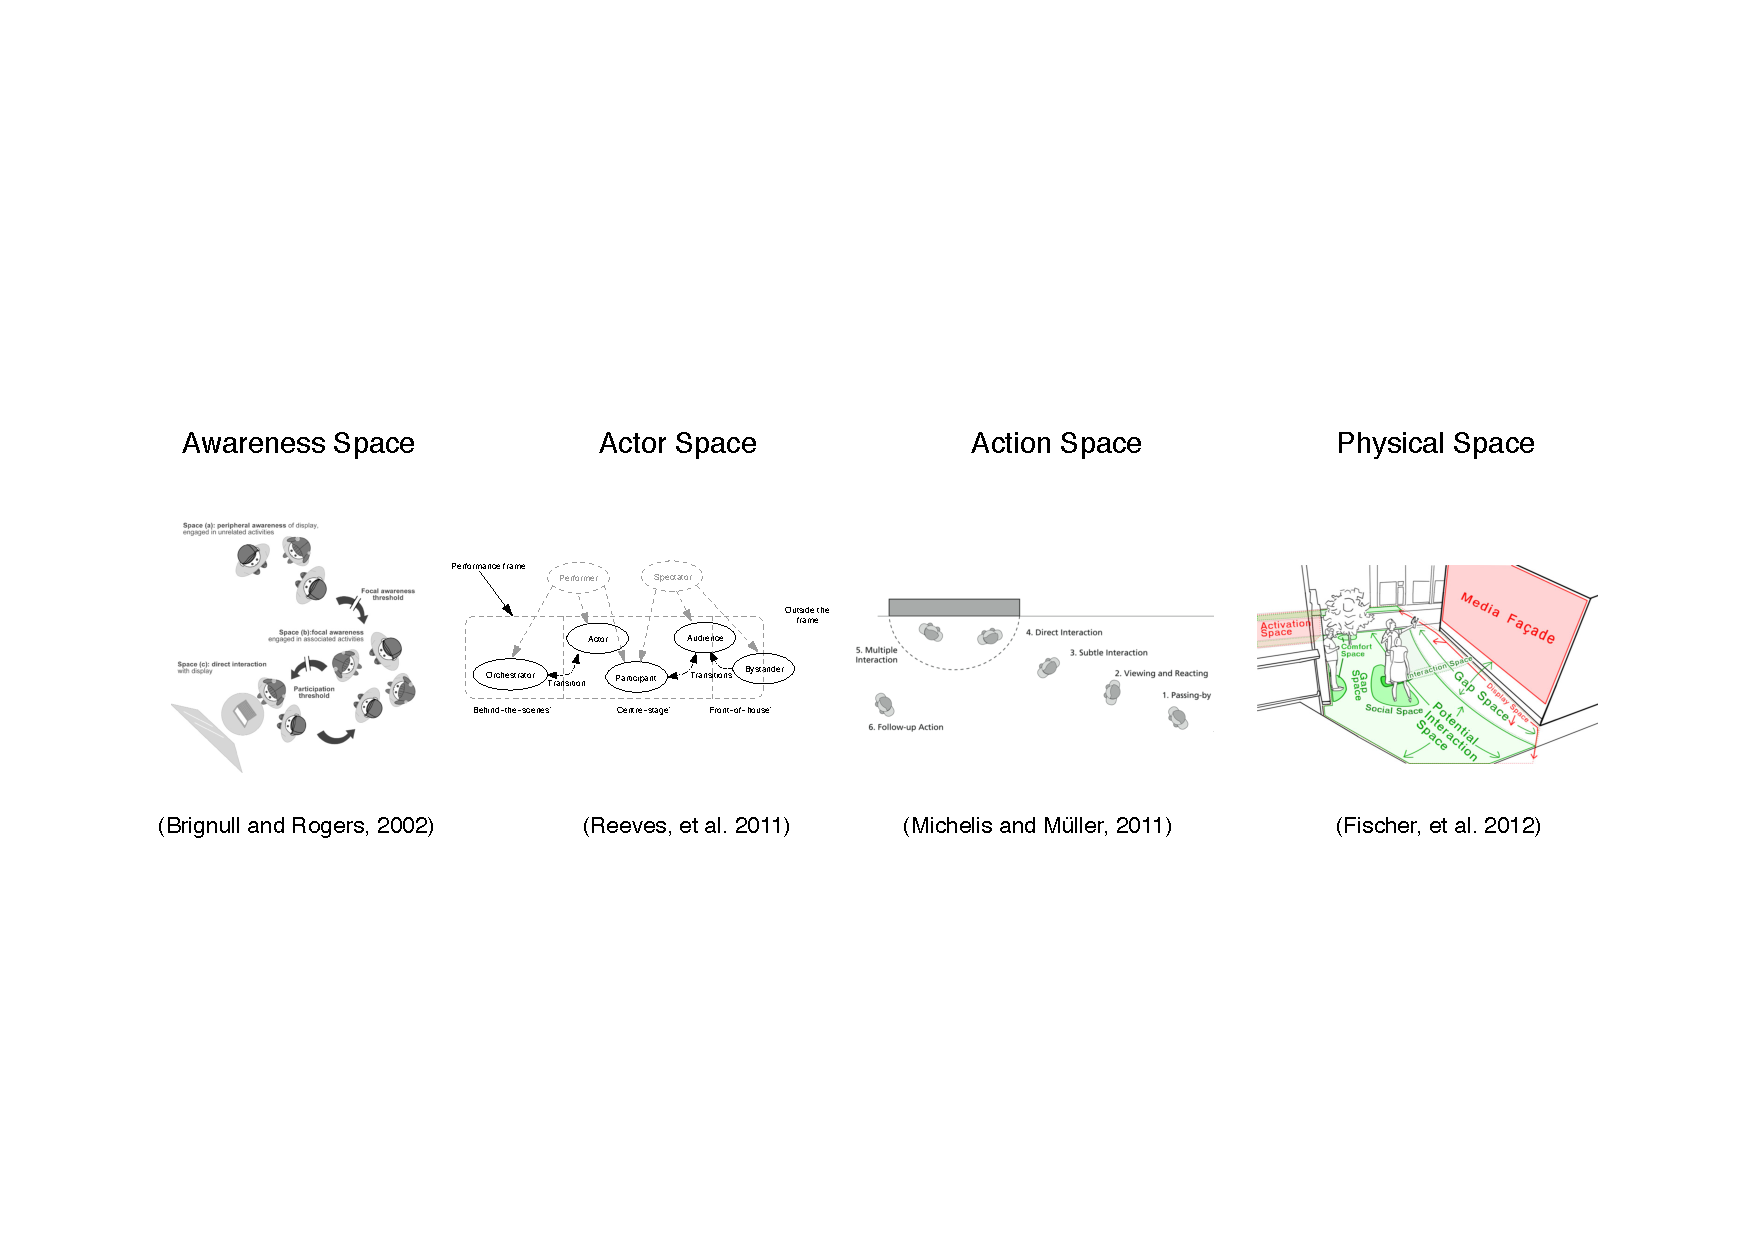
\includegraphics[width=\textwidth]{Illustrations/SpatialFrameworks.pdf}
\caption{Four existing socio-spatial interaction frameworks}
\label{fig:Background-frameworks}
\end{figure}

%%%%%%%%%%%%%%%%%%%%%%%%%%%%%

\subsection* {Awareness Space}
Research on awareness of public displays in relation to social interactions was first described in HCI research, when noticing a novel social phenomenon around public displays (Brignull and Rogers 2003). 
Three different types of ‘activity spaces’ were described: (1) Peripheral awareness activities: activities that take place in the wider space around the display, where people socialize but are not necessarily aware of the presence of the public display. (2) Focal awareness activities: in this space, people are aware of the presence of the display. 
They are looking at the display, discuss activities that take place around the display or learn how to engage with the content. (3) Direct interaction activities: this is the space where individuals or groups actively engage with the display. The research findings suggest that
people found it difficult to transit from one ‘activity space’ to another.
Later, Vogel and Balakrishnan (2004) published a spatial framework, which
described how users fluidly move from implicit interactions in the wider surrounding
towards explicit interactions when approaching the direct interaction space
around a public display.

\subsection* {Actor Space}
The actor space describes the different roles people take on when being in the vicinity of interactive installations. 
By now, computers have moved away from the desktop and novel interfaces appear, which spread into new spatial settings.
People are changing their role; in particular, in public settings people traverse various awareness spaces, which afford specific roles. 
Consequently, a better understanding of what kind of roles these are, when and where people take them on, is crucial for the design and deployment of interactive systems in urban spaces.
Reeves (2011) identified that the conventional user is actually changing her role when passing-by, on looking or turning into a performer in the vicinity of an interactive installation. 
Within this framework, the performing user plays the central role when engaging with an interface. 
Her acting entices other people from the audience into the experience; some of them may become performers. 
More recently, Behrens et al. (2013), and Fatah gen Schieck et al. (2013), have explored in detail how these roles are framed through the situated layout of urban screens.

\subsection* {Action Space}
In the last section, we clarify the diverse roles individuals take on in connection with interactive installations; here, we describe the various phases of interactions people traverse. 
The Audience Funnel by Michelis and Müller (2011) depicted a framework that establishes a terminology for each transition. 
These phases were identified as (1) passing by, (2) viewing and reacting, (3) subtle interaction, (4) direct interaction, (5) multiple interactions and (6) follow-up action. 
Michelis and Müller found that people proceed from one phase to the next in order to understand the interaction. 
Boundaries are described as a series of thresholds that need to be crossed before one can interact with a public display.

\subsection* {Physical Space}
The spatial localization of interactions is largely neglected in the work described above. 
In contrast, Fischer and Hornecker (2012) have outlined an interaction framework that focuses on the spatial properties of interactions. 
When looking into the various encounter stages, ‘urbanHCI’ specifies different ‘interaction spaces’ on which people perform different activities. 
This includes the (1) display spaces, (2) interaction spaces, (3) potential interaction spaces, (4) gap spaces, (5) social interaction space, (6) comfort space and (7) activation space on which participants
behave differently towards an interactive media facade. 
Fischer and Hornecker’s framework was explored through a media art project called ‘SMSlingshot’. 
This project developed an interface that looks like a wooden slingshot, but its integrated digital technology allows the user to shoot short text messages (SMS) together with virtual paintballs on a media facade. 
Within these immediate spaces around an electronic display (i.e. interaction spaces), passers-by stop, watch and start playing with the media architectural interface and eventually change the look of the media façade individually; others observe in groups from a distance, discuss or engage as well; simultaneously, other pedestrians do not sense the presence of such interactions and the existence of the media facade at all. 
‘Screens in the Wild’, on the other hand, addressed the question of spatial layout and its relation to technologically mediated interactions (Behrens et al. 2013; Fatah gen Schieck et al. 2013). 
Four interactive and networked urban screens have been deployed in four different neighbourhoods in London and Nottingham.
Within this approach, the following interaction zones were recognized: (1) direct interaction space surrounding the display (direct); (2) the surrounding public space (wide); and (3) across spatial boundaries, i.e. the remotely connected space through the networked displays (networked).
Sociospatial configurations mediated by urban screens were explored, and site-specific interactions were observed and compared to more generic types of interactions. 
Indications were found that the properties of the spatial layout play a significant role and, to a certain extent, frame the type of interactions mediated through public displays (Fig. 2).

In a more systematically approach the ‘Screens in the Wild’ research project explored socio-spatial configurations mediated by urban screens (Behrens et al. 2013, Fatah et al. 2013). Within this research project four interactive and networked urban screens have been deployed in four different neighbourhoods in London and Nottingham. The particular study the applied methodology, included the analysis of the spatial layout in two screen locations in London. This was followed by the observations of social behaviour and technologically mediated interactions by actors, spectators and passers-by during two community events. Within this study the following interaction zones were recognized: 1) direct interaction space surrounding the display (direct); 2) the surrounding public space (wide); and 3) across spatial boundaries i.e. the remotely connected space through networked displays (connected) over time. Site-specific interactions were observed and compared to more generic types of interactions. Indications were found, that the properties of the spatial layout play a significant role and, to a certain extent, frame the type of interactions mediated through public displays (fig. 34).

%%%%%%%%%%%%%%%%%%%%%%%%%%%%%

\begin{figure}[htp]
\centering
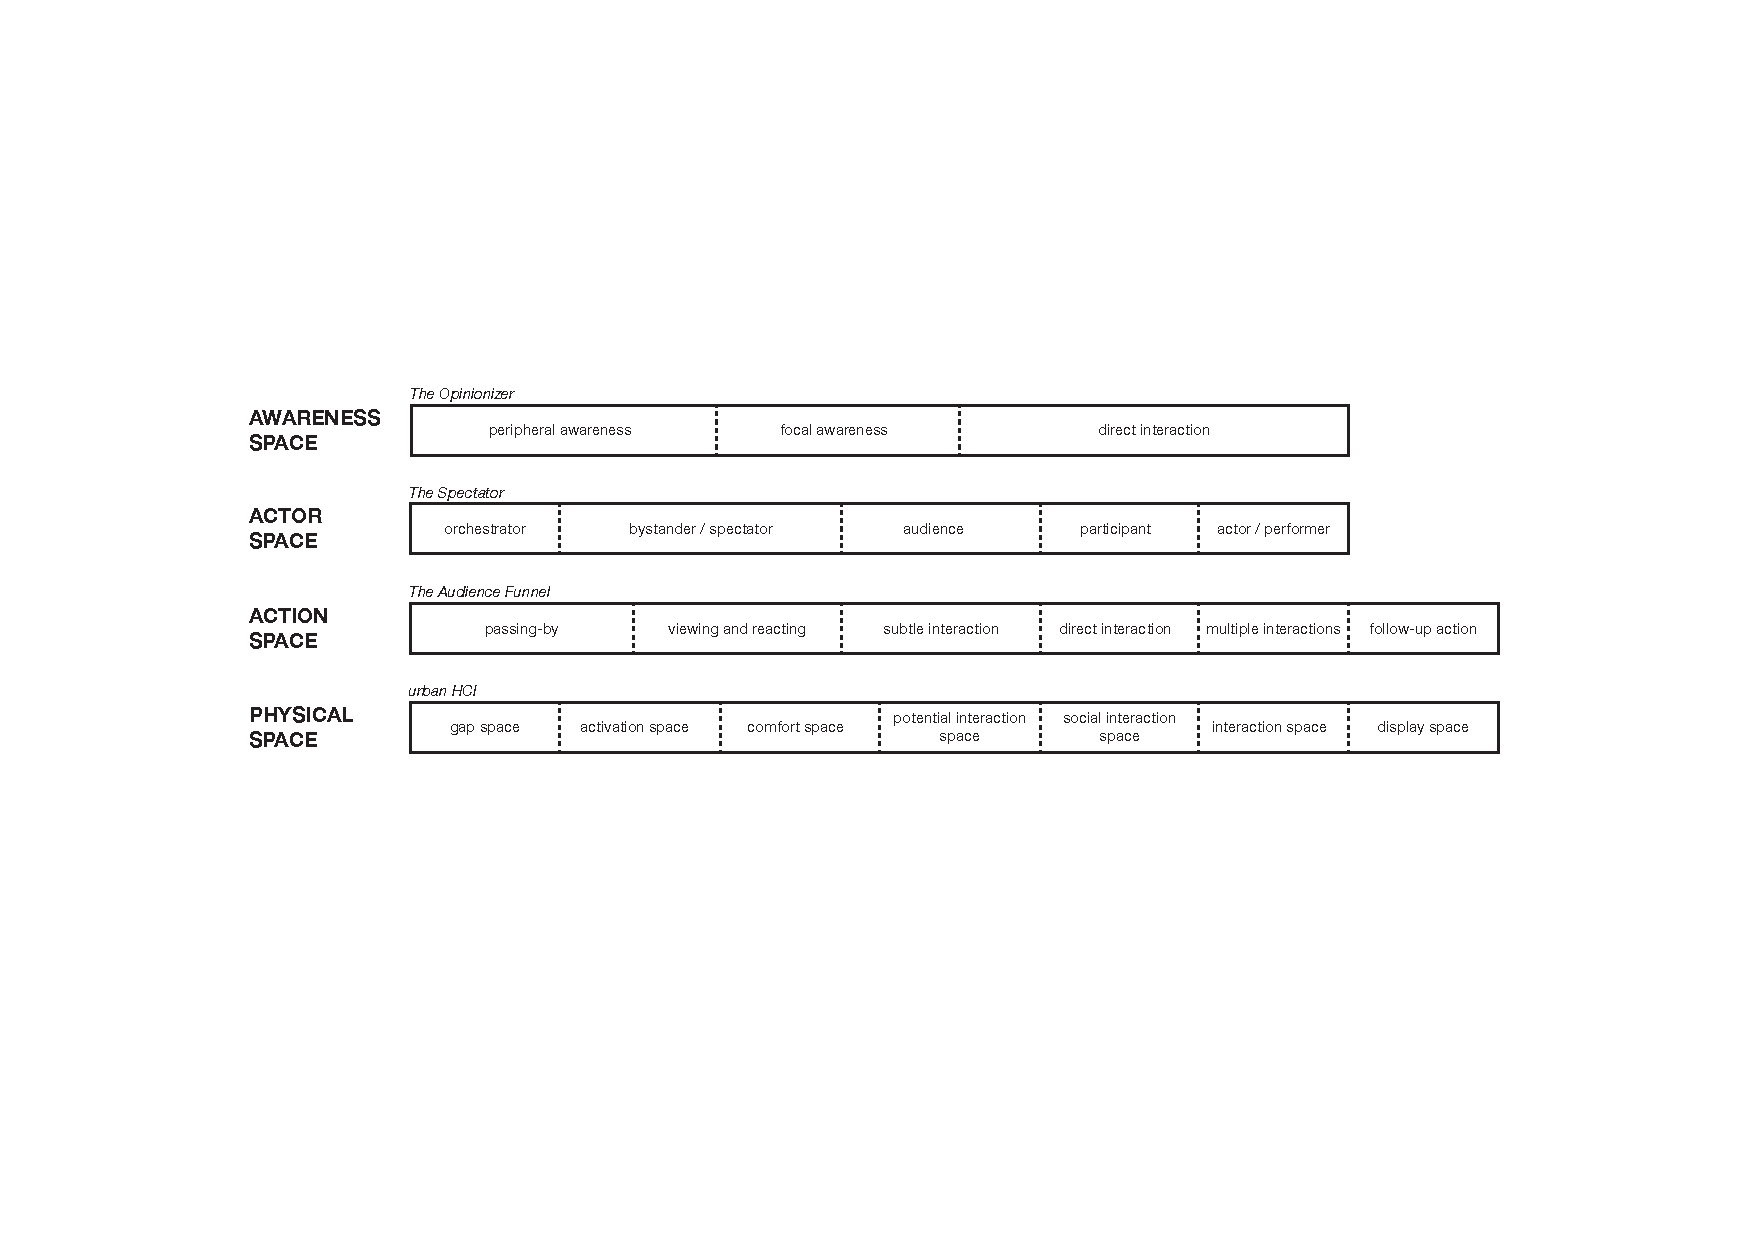
\includegraphics[width=\textwidth]{Illustrations/SpatialFrameworks_2.pdf}
\caption{Comparison of four spatial frameworks for describing interaction mediated through public
displays}
\label{fig:comparison}
\end{figure}

%%%%%%%%%%%%%%%%%%%%%%%%%%%%%

In summary, we plotted four existing spatial frameworks that describe interactions between humans and displays from (1) awareness spaces, (2) actor spaces, (3) action spaces and (4) physical spaces. 
Although three of the presented frameworks dealt with smaller public displays, in comparison with the large urban displays, juxtaposing these frameworks assists designers to understand the multilayered design space when designing interactive systems for large programmable displays. 
We contribute to this body of research by exploring specifically the relation between TUI and large programmable displays (such as media facades) in a given context. We clarify the notion of MAI and apply it on two design case studies we conducted.

%%%%%%%%%%%%%%%%%%%%%%%%%%%%%

%\begin{figure}[htp]
%\centering
%\includegraphics[width=\textwidth]{IMG_3399Resized_Image_1024}
%\caption{ShareLaTeX logo}
%\label{fig:lion}
%\end{figure}

%%%%%%%%%%%%%%%%%%%%%%%%%%

\section {Towards Sentiment Architectures}

Sentiment Architectures are a specific type of Media Architectures


A panopticon that allows for its inmates to be visually observed at any time is a Sentiment Architecture. 
A fortified panic room that provides shelter for people to take refuge in case of a threat is a Sentiment Architecture. 
A participatory media installation is a Sentiment Architecture. 
Sentiment Architecture is not a typology.
It is a function. That is why we use its plural, Sentiment Architectures.
The term is derived from a technology called sentiment analysis — a tool to identify people’s emotions in language. 
The contents of this book try to utilise this idea and its potential for an expanded architectural theory and practice. 
Following this approach, Sentiment Architectures are not either positive or negative. 
They are part of our world. They are part of us. 
And that is why we have to attain a conscious understanding and handling of them. 
This is what this collage-like publication is aiming for.
It meanders through a variety of forms to encounter this phenomenon in all its modes of existence: A socio-critical utopia, a subjective history, a real-world documentation, a satellite essay, an individual mythology, and two interviews create a picture of our world where subject and object collided and fused into one a long time ago. 
We think it is about time for architecture to acknowledge that more actively.

%%%%%%%%%%%%%%%%%%%%%%%%%%%

\section {Discussion}

Having reviewed research on public spaces it is clear that human behaviour and social interactions are in the focus when designing.

%%%%%%%%%%%%%%%%%%%%%%%%%%%%%

Today it is all about the understanding of human behaviour.

%%%%%%%%%%%%%%%%%%%%%%%%%%%%%

\begin{singlespace}
	\leftskip2.3em
		\rightskip\leftskip
			\textit{\small Public realm considerations are our most powerful tool in designing cities that work for their inhabitants. In order to create and enhance vital, functional public spaces, we need to gain a better understanding of the way different demographic groups want to use and experience the city.}
	
    \small ARUP, Cities Alive - Rethinking the Shades of Night.\\
\end{singlespace}

%%%%%%%%%%%%%%%%%%%%%%%%%%%%%

In recent years the socio-economic relationship between so called 'good' public spaces and quality of life in urban areas has become the focus for those responsible such as politicians, urban planners, architects, local neighbourhood initiatives and more recently for businesses.  
Already in 1997 this had led to the economic assumption by The Department of the Environment, UK:

\begin{singlespace}
	\leftskip2.3em
		\rightskip\leftskip
			\textit{\small For retailers, a good-quality public environment can improve trading by attracting more people into an area. It has been shown, for example, that well-planned improvements to public spaces within town centres can boost commercial trading by up to 40 per cent and generate significant private sector investment. Urban design improvements undertaken as part of a wider strategy can have even more dramatic results.\footnote{in: DoE and The Association of Town Centre
Management (1997) Managing Urban Spaces in Town Centres – Good Practice Guide. London, HMSO taken from: The Value of Public Space: How high quality parks and public spaces create economic, social and environmental value, by CABE Space. 2014. Available from: http://www.designcouncil.org.uk/sites/default/files/asset/document/the-value-of-public-space1.pdf; accessed 19.10.2016}}
\end{singlespace}

Of course that raises immediately the question what a 'good-quality public environment' constitutes?

%%%%%%%%%%%%%%%%%%%%%%%%%%%
